\documentclass[12pt,aspectratio=169]{beamer}

% ====================================================
% ====================================================
% USEPACKAGES AND IMPORTS
% ====================================================
% ====================================================

\usepackage[T1]{fontenc}
\usepackage[utf8]{inputenc}
\usepackage[english]{babel}

% tables
\usepackage{tabularx}
\usepackage{colortbl}
\usepackage{multirow}
\usepackage{makecell}

% tikz and colors
\usepackage{tikz}
\usepackage{xcolor}
\usepackage{pgfplots}
\usepackage{pgfplotstable}
\usepackage{tikzsymbols}

\usetikzlibrary{calc}
\usetikzlibrary{trees}
\usetikzlibrary{patterns}
\usetikzlibrary{shadings}
\usetikzlibrary{positioning}
\usetikzlibrary{intersections}
\usepgfplotslibrary{patchplots}
\usepgfplotslibrary{fillbetween}
\usetikzlibrary{decorations.pathreplacing}

\usetikzlibrary{arrows}
\usetikzlibrary{arrows.meta}

\usetikzlibrary{shapes}
\usetikzlibrary{shapes.arrows}
\usetikzlibrary{shapes.callouts}
\usetikzlibrary{shapes.symbols}
\usetikzlibrary{shapes.geometric}

% boxes
\usepackage[many]{tcolorbox}

% math packages and fonts
\usepackage{bm}
\usepackage{ccfonts}
\usepackage{eulervm}
\usepackage{amsmath}
\usepackage{amsfonts}
\usepackage{amssymb}
\usepackage{amsthm}
\usepackage{mathtools}
\usepackage{nicefrac}
\usepackage{slashed}
\usepackage{bbold}
\usepackage{array}
\usepackage{cancel}

% algorithms and listings
\usepackage[ruled,vlined,linesnumbered]{algorithm2e}
\usepackage{listings}
\usepackage{setspace}

\tcbuselibrary{listings}
\tcbuselibrary{breakable}
\tcbuselibrary{skins}

% misc
\usepackage{soul}
\usepackage{pifont}
\usepackage{skull}
\usepackage{multicol}
\usepackage{animate}
\usepackage{hyperref}
\usepackage{wasysym}
\usepackage[absolute,overlay]{textpos}
\usepackage[hang,flushmargin]{footmisc}

% ====================================================
% ====================================================
% LAYOUT AND THEME
% ====================================================
% ====================================================

\usetheme{Copenhagen}

% color definitions
\definecolor{myblue1}{RGB}{35,119,189}
\definecolor{myblue2}{RGB}{95,179,238}
\definecolor{myblue3}{RGB}{129,168,207}
\definecolor{myblue4}{RGB}{26,89,142}

\definecolor{myred1}{RGB}{247,12,12}

% set theme colors
\setbeamercolor*{structure}{fg=myblue1,bg=blue}
\setbeamercolor*{palette primary}{use=structure,fg=white,bg=structure.fg}
\setbeamercolor*{palette secondary}{use=structure,fg=white,bg=structure.fg!75!black}
\setbeamercolor*{palette tertiary}{use=structure,fg=white,bg=structure.fg!50!black}
\setbeamercolor*{palette quaternary}{fg=black,bg=white}

\setbeamertemplate{itemize item}[circle]
\setbeamertemplate{itemize subitem}[circle]
\setbeamertemplate{itemize subsubitem}[circle]

\setbeamertemplate{enumerate item}[circle]
\setbeamertemplate{enumerate subitem}[circle]
\setbeamertemplate{enumerate subsubitem}[circle]

\setbeamercolor{itemize item}{fg=myblue1}
\setbeamercolor{itemize subitem}{fg=myblue1}
\setbeamercolor{itemize subsubitem}{fg=myblue1}

\setbeamertemplate{section in toc}[circle]
\setbeamertemplate{subsection in toc}[circle]
\setbeamerfont{subsection in toc}{size=\scriptsize}

\setbeamercolor{frametitle continuation}{fg=black}

% title graphic -- sap logo and dhbw logo
\titlegraphic{
\includegraphics[scale=0.1]{../03_img/logo_sap}\hspace*{4.75cm}~%
   	
\includegraphics[scale=0.05]{../03_img/logo_dhbw}
}

\makeatletter
% frame title
\defbeamertemplate*{frametitle}{mydefault}[1][left]
{
  	\ifbeamercolorempty[bg]{frametitle}{}{\nointerlineskip}%
  	\nointerlineskip%
 	\@tempdima=\textwidth%
  	\advance\@tempdima by\beamer@leftmargin%
  	\advance\@tempdima by\beamer@rightmargin%
  	\begin{tcolorbox}[
  		enhanced,
  		outer arc=0pt,
  		arc=0pt,
  		boxrule=0pt,
  		top=0pt,
  		bottom=0pt,
  		enlarge left by=-\beamer@leftmargin,
  		enlarge right by=-\beamer@rightmargin,
  		width=\paperwidth,
  		nobeforeafter,
  		interior style={
    			left color=myblue2,
    			right color=white
    		},
  		shadow={0mm}{-0.4mm}{0mm}{black!60,opacity=0.6},    
  		shadow={0mm}{-0.8mm}{0mm}{black!40,opacity=0.4},    
  	]
    	\usebeamerfont{frametitle}%
    	\vbox{}\vskip-1ex%
    	\if@tempswa\else\csname beamer@fte#1\endcsname\fi%
    	\insertframetitle\par%
    	{%
      		\ifx\insertframesubtitle\@empty%
      		\else%
      		{\usebeamerfont{framesubtitle}\usebeamercolor[fg]{black}\insertframesubtitle\strut\par}%
      		\fi
    	}%
    	\vskip-1ex%
    	\if@tempswa\else\vskip-.3cm\fi
  	\end{tcolorbox}%
}

% footline of a frame
\defbeamertemplate*{footline}{mysplit theme}
{%
  	\leavevmode%
  	\hbox{
		\begin{beamercolorbox}[
			wd=.5\paperwidth,ht=2.5ex,dp=1.125ex,leftskip=.3cm plus1fill,rightskip=.3cm
		]{author in head/foot}%
    			\usebeamerfont{author in head/foot}\insertshortauthor\ (\insertinstitute), \insertdate
  		\end{beamercolorbox}%
  		\begin{beamercolorbox}[
			wd=.5\paperwidth,ht=2.5ex,dp=1.125ex,leftskip=.3cm,rightskip=.3cm plus1fil
		]{title in head/foot}%
    			\usebeamerfont{title in head/foot}\insertshorttitle\hfill
    			\insertprefix-\insertframenumber/\inserttotalframenumber\hspace*{0.5em}
  		\end{beamercolorbox}}%
  	\vskip0pt%
}
\makeatother

% ====================================================
% ====================================================
% COMMANDS AND GENERAL DEFINITIONS
% ====================================================
% ====================================================

% page number prefix
\newcommand\insertprefix{}  % empty by default
\newcommand\prefix[1]{\renewcommand\insertprefix{#1}}

% math definitions
% ====================================================
\DeclareMathOperator*{\argmax}{arg\,max}
\DeclareMathOperator*{\argmin}{arg\,min}
\newcommand*\diff{\mathop{}\!\mathrm{d}}

\newcommand*{\vertbar}{\rule[-1ex]{0.5pt}{2.5ex}}
\newcommand*{\horzbar}{\rule[.5ex]{2.5ex}{0.5pt}}

% commands
% ====================================================

% highlight commands
% --------------------------------------------------------------------------------------------------------
% highlight command
\newcommand{\highlight}[1]{\textcolor{myblue1}{\textbf{#1}}}
\newcommand{\highlighttt}[1]{\textcolor{myblue1}{\texttt{#1}}}
\newcommand{\Highlight}[1]{\textcolor{myred1}{\textbf{#1}}}

% blue color boxes (with frame/without frame/without fill)
\newtcolorbox{boxBlue}{colback=myblue1!10!white,colframe=myblue4}
\newtcolorbox{boxBlueNoFrame}{colback=myblue1!10!white,colframe=myblue1!10!white}
\newtcolorbox{boxBlueNoFill}{colback=white,colframe=myblue4}

% font commands
% --------------------------------------------------------------------------------------------------------
\newcommand{\linkstyle}[1]{\underline{\smash{\texttt{#1}}}} 		% style of hyperlinks

% tikz commands
% --------------------------------------------------------------------------------------------------------

% yellow sticky note
\newcommand{\bubble}[3]{
\begin{textblock}{100}(#1, #2)
      	\begin{tikzpicture}
		\node[rectangle,draw=yellow,very thick,fill=yellow!60,align=center] at (0,0) {#3};
	\end{tikzpicture}
\end{textblock}
}

\newcommand{\floattext}[3]{
\begin{textblock}{100}(#1, #2)
      	#3
\end{textblock}
}

\newcommand{\doublecircle}[2]{
	\draw[fill=white,draw=myblue1] (#1,#2) circle (2mm);
	\draw[fill=myblue1,draw=myblue1] (#1,#2) circle (1.5mm);
}

% slide modifiers
% --------------------------------------------------------------------------------------------------------
% mark slide as optional
\newcommand{\optional}{
	\begin{textblock}{100}(0.15,0.30)
      		
\includegraphics[scale=0.2]{../03_img/scream}
    	\end{textblock}
}

% mark slide as important
\newcommand{\important}{
	\begin{textblock}{100}(0.10,0.15)
      		
\includegraphics[scale=0.1]{../03_img/important}
    	\end{textblock}
}

% citation
% --------------------------------------------------------------------------------------------------------
% first argument in {book, online, article}
\newcommand{\literature}[5]{
	\setbeamertemplate{bibliography item}[#1]
	\bibitem{#2}
	\highlight{#3} \\
	\textcolor{darkgray}{\textit{#4}} \\
	\textcolor{black}{#5}
}
% cite content
\newcommand{\citeAuthor}[3]{\vfill\scriptsize\textcolor{lightgray}{#1 \cite{#2} #3}}

% slide architecture
% --------------------------------------------------------------------------------------------------------
% divide frame into two parts
\newcommand{\divideTwo}[4]{
	\begin{minipage}{#1\textwidth}
		#2
	\end{minipage}
	\hfill
	\begin{minipage}{#3\textwidth}
		#4
	\end{minipage}
}

% divide frame into two parts (start on top)
\newcommand{\divideTwoTop}[4]{
	\begin{minipage}[t]{#1\textwidth}
		#2
	\end{minipage}
	\hfill
	\begin{minipage}[t]{#3\textwidth}
		#4
	\end{minipage}
}

% special pages
% --------------------------------------------------------------------------------------------------------
% title page
\newcommand{\maketitlepage}{
	{
		\beamertemplatenavigationsymbolsempty
		\usebackgroundtemplate{%
			\tikz[overlay,remember picture] \node[opacity=0.2, at=(current page.center)] {
  				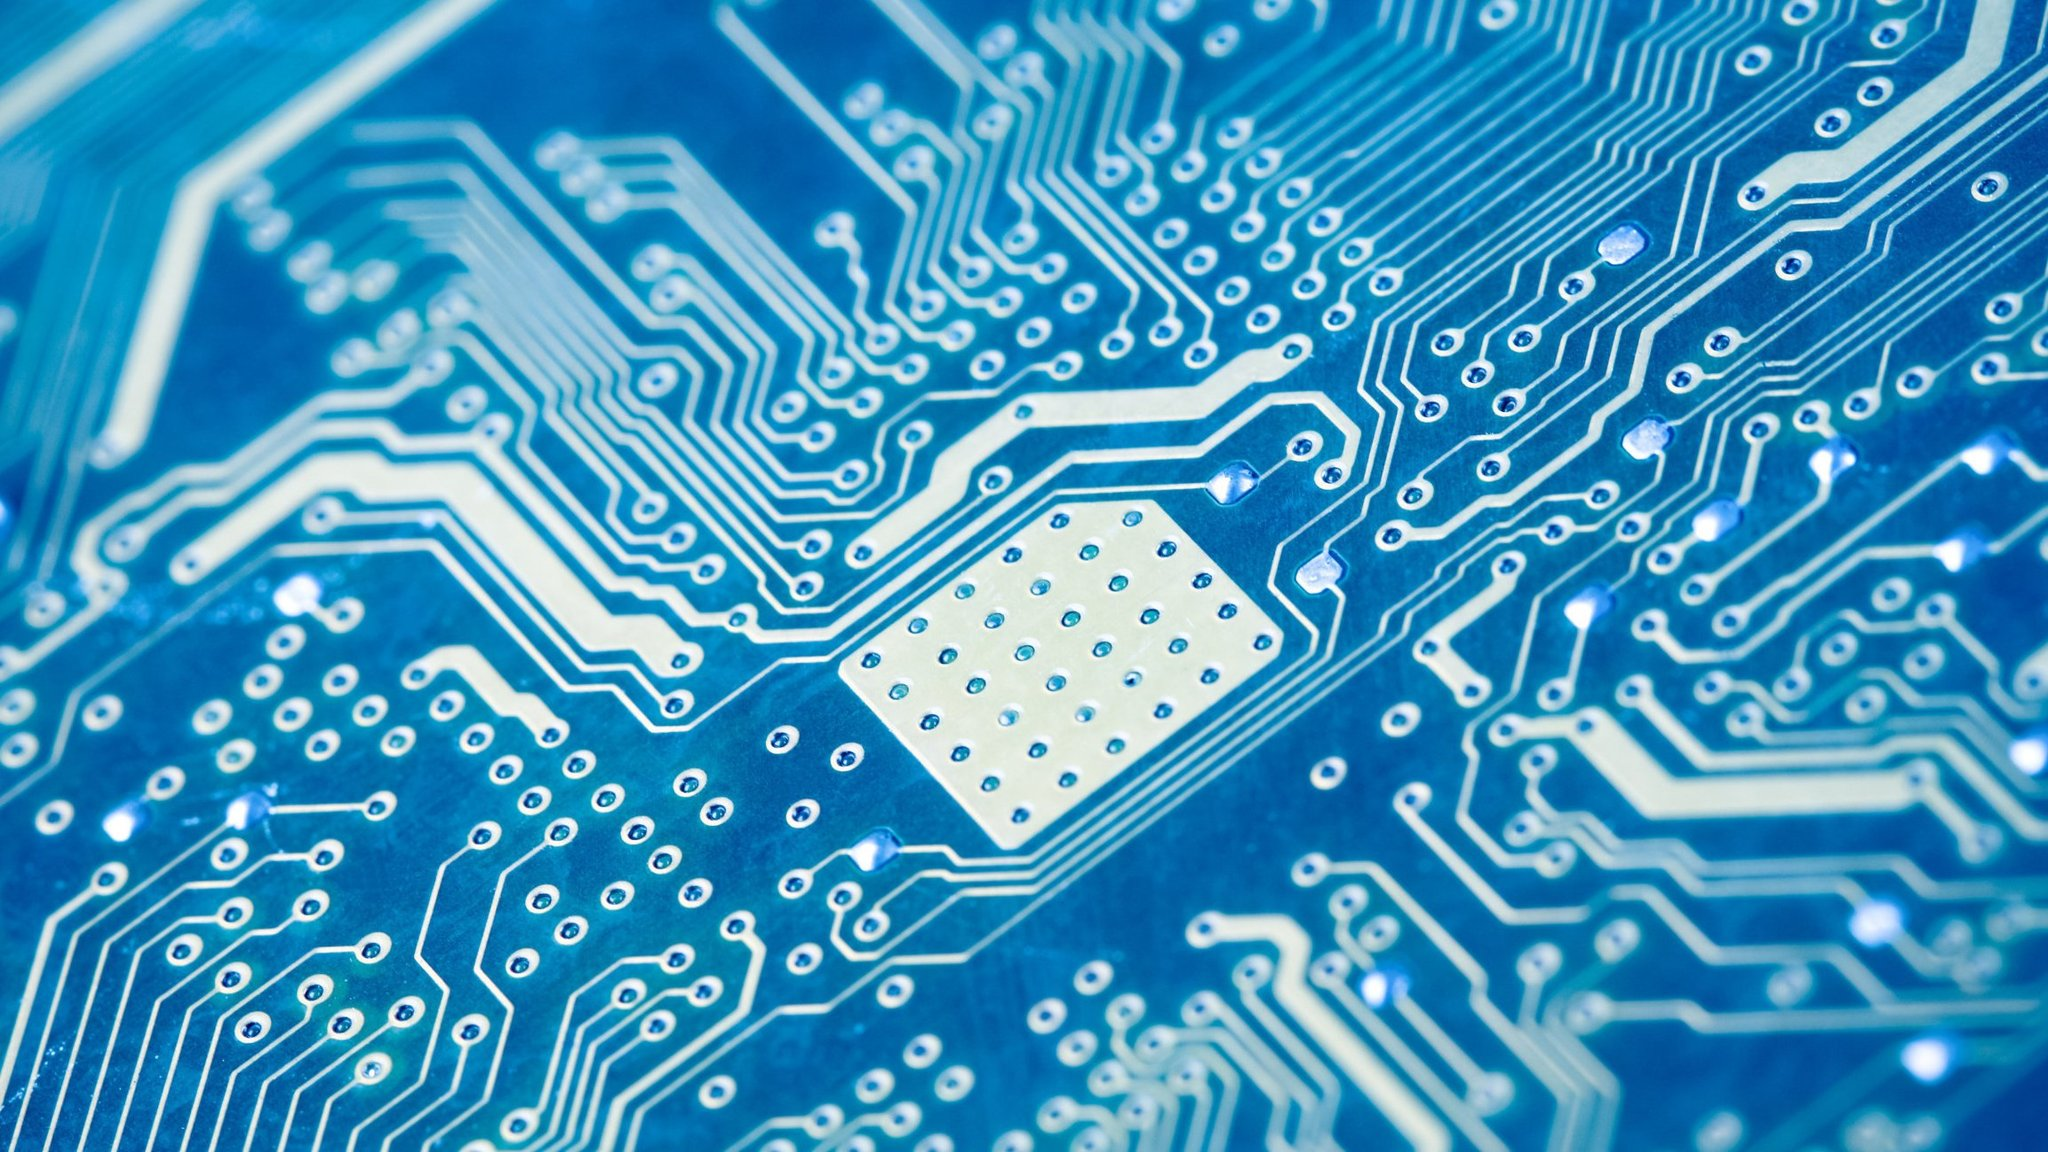
\includegraphics[height=\paperheight,width=\paperwidth]{../03_img/processor.jpg}
			};
		}
		\begin{frame}[plain]
			\vspace*{0.75cm}
			\maketitle
			\vfill
			\begin{center}
				\footnotesize Find all slides on \href{https://github.com/DaWe1992/Applied_ML_Fundamentals}{\linkstyle{GitHub}}
			\end{center}
		\end{frame}
	}
}

% divider page
\newcommand{\makedivider}[1]{
	{
		\beamertemplatenavigationsymbolsempty
		\usebackgroundtemplate{%
			\tikz[overlay,remember picture] \node[opacity=0.2, at=(current page.center)] {
  				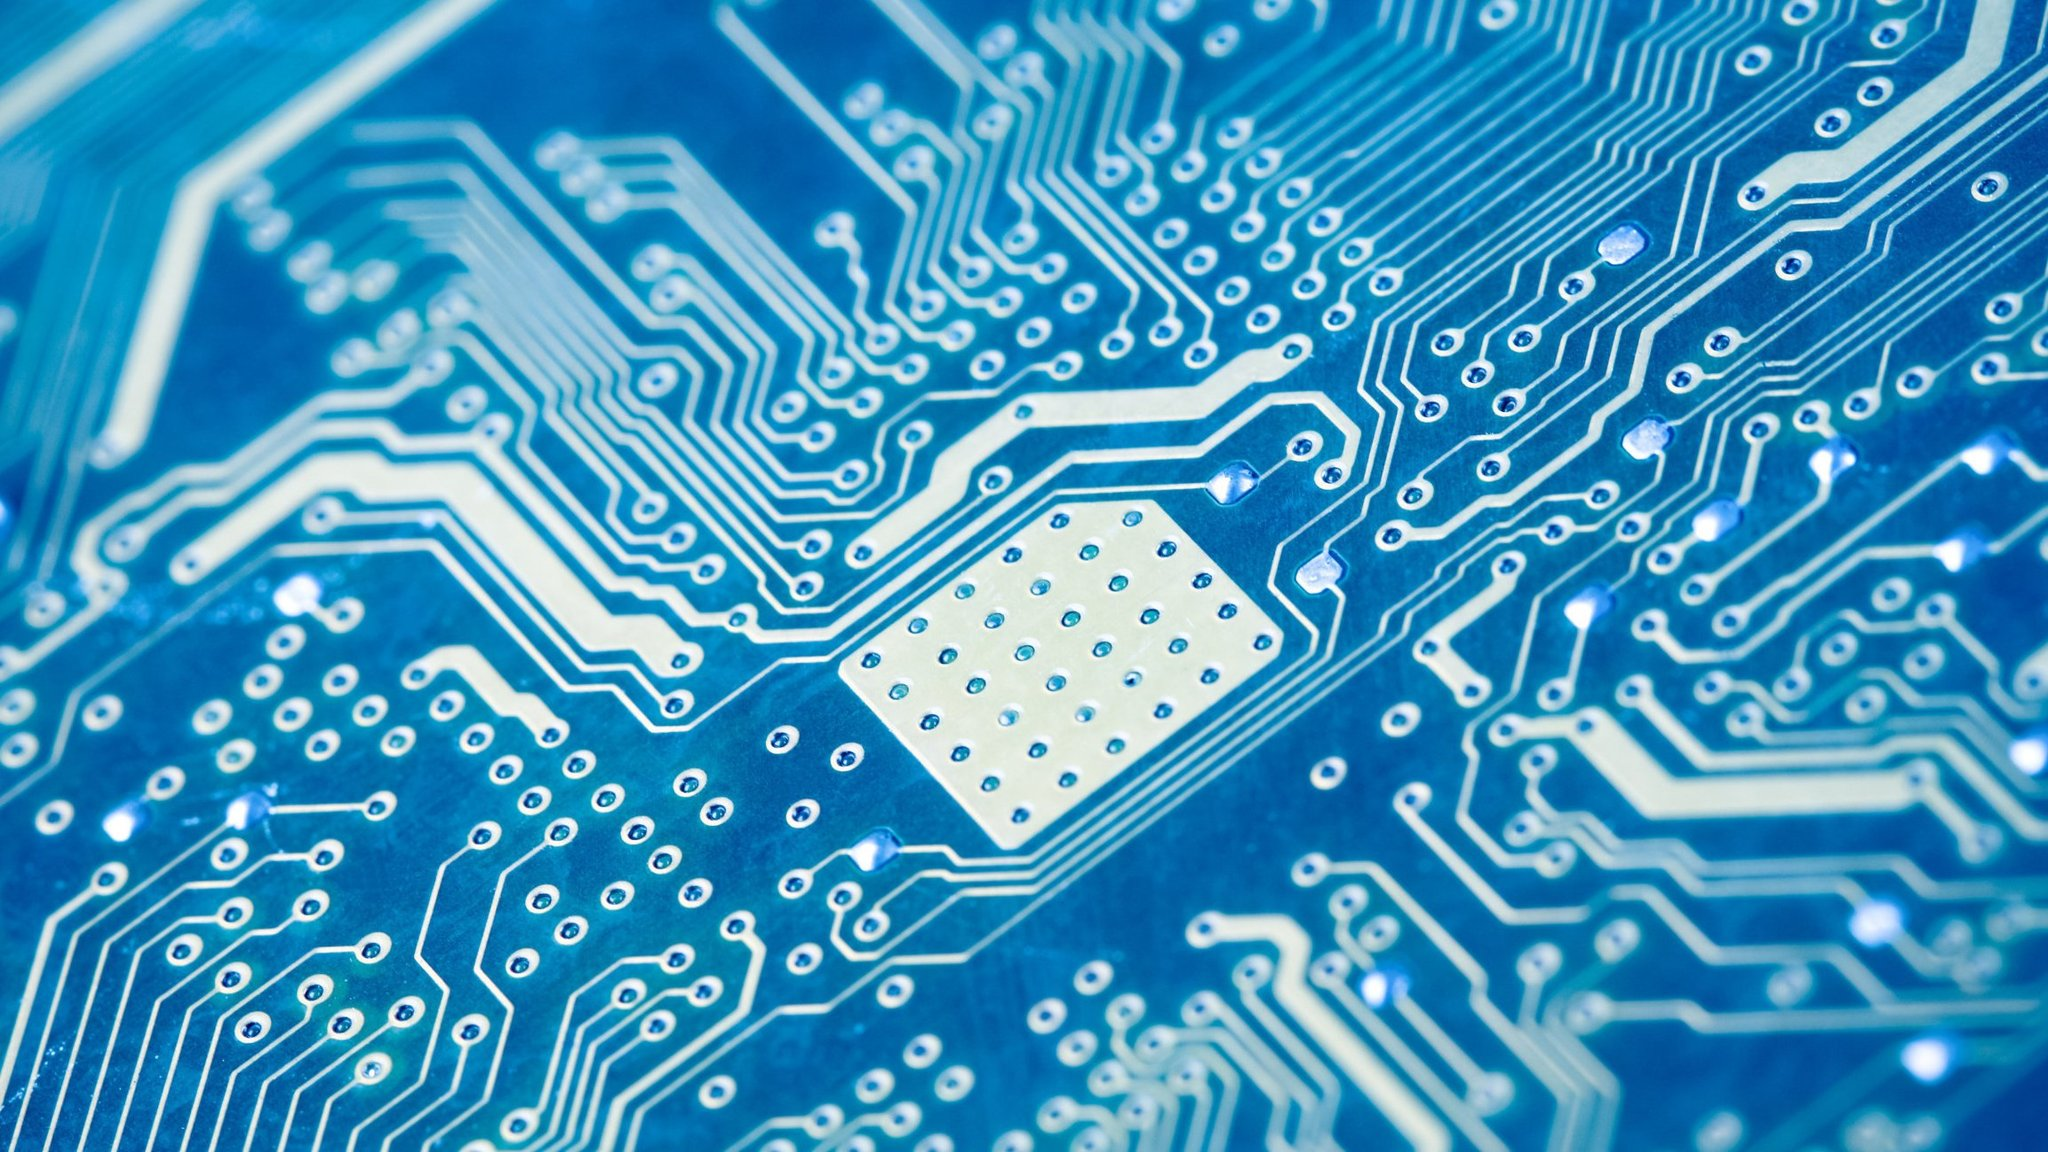
\includegraphics[height=\paperheight,width=\paperwidth]{../03_img/processor.jpg}
			};
		}
		\begin{frame}[plain]
			\vfill
			\begin{boxBlue}
				\centering
				\textbf{Section:} \\
				\large \highlight{#1}
			\end{boxBlue}
			\vfill
			\centering
			
\includegraphics[scale=0.05]{../03_img/logo_dhbw.png}
			\vfill
		\end{frame}
	}
}

% overview page
\newcommand{\makeoverview}[1]{
	\begin{frame}{Lecture Overview}{}
		\begin{tabbing}
			\hspace*{3.5cm}\= \kill
			\ifnum #1=1 \highlight{\textbf{Unit I:}} \else \textbf{Unit I:} \fi
			\> \ifnum #1=1 \highlight{Machine Learning Introduction} \else Machine Learning Introduction \fi \\
		\end{tabbing}
	\end{frame}
}

% thank you page
\newcommand{\makethanks}{
	{\beamertemplatenavigationsymbolsempty
	\begin{frame}[plain]
		\vfill
		\begin{boxBlue}
			\centering
			\Large \highlight{Thank you very much for the attention!}
		\end{boxBlue}
		
		\vfill\footnotesize
		\begin{tabbing}
			\hspace*{1.5cm}\= \kill
			\highlight{Topic:} 	\> \inserttitle \\
			\highlight{Date:} 	\> \insertdate
		\end{tabbing}
		
		\vfill
		\highlight{Contact:} \\
		\insertauthor\ (D062271) \\
		\insertinstitute \\
		\href{mailto:daniel.wehner@sap.com}{\linkstyle{daniel.wehner@sap.com}}
		
		\vfill\normalsize
		\begin{center}
			\large\highlight{Do you have any questions?}
		\end{center}
		\vfill
	\end{frame}}
}

% global pfgplots settings
% --------------------------------------------------------------------------------------------------------
\pgfplotsset{
	% allow filtering of data for pgfplots
	discard if/.style 2 args={
        		x filter/.code={
            		\edef\tempa{\thisrow{#1}}
            		\edef\tempb{#2}
            		\ifx\tempa\tempb
                		\def\pgfmathresult{inf}
            		\fi
        		}
    	},
    	discard if not/.style 2 args={
        		x filter/.code={
            		\edef\tempa{\thisrow{#1}}
            		\edef\tempb{#2}
            		\ifx\tempa\tempb
            		\else
                		\def\pgfmathresult{inf}
            		\fi
        		}
    	}
}


% ====================================================
% ====================================================
% PRESENTATION DATA
% ====================================================
% ====================================================

\title[Probability Density Estimation]{*** Applied Machine Learning Fundamentals *** Probability Density Estimation (PDE)}
\institute[SAP\,SE]{SAP\,SE / DHBW Mannheim}
\author{Daniel Wehner, M.Sc.}
\date{Winter term 2020/2021}
\prefix{PDE}

% ====================================================
% ====================================================
% BEGIN OF DOCUMENT
% ====================================================
% ====================================================

\begin{document}

% Title frame
%______________________________________________________________________
\maketitlepage


% Lecture Overview
%______________________________________________________________________
\begin{frame}{Lecture Overview}{}
	\makeoverview{4}
\end{frame}


% Agenda
%______________________________________________________________________
\begin{frame}{Agenda for this Unit}
	\begin{multicols}{2}
		\tableofcontents
	\end{multicols}
\end{frame}


% Section: Introduction
%______________________________________________________________________
\section{Introduction}
\makedivider{Introduction}

% Subsection: 
% --------------------------------------------------------------------------------------------------------
\subsection{What about continuous Data?}

% Probability Density Estimation (PDE)
\begin{frame}{Probability Density Estimation (PDE)}{}
	\begin{itemize}
		\item We have learned about Bayes' optimal classifiers which classify data based on the probability distribution
			$p(\bm{x} \vert \mathcal{C}_k) \cdot p(\mathcal{C}_k)$
		\item (Multinomial) Na\"{i}ve Bayes is an instance of PDE for \textbf{discrete data}
		\item \highlight{How to get these probabilities in the continuous case?}
		\begin{itemize}
			\item The prior $p({\mathcal{C}_k})$ is still easy to compute
			\item The estimation of class conditional probabilities $p(\bm{x} \vert \mathcal{C}_k)$ is more complicated
			\item Assume labeled data; estimate the density separately for each class $\mathcal{C}_k$
		\end{itemize}
		\item NB: For ease of notation: $p(x) \equiv p(x \vert \mathcal{C}_k)$
	\end{itemize}
\end{frame}


% Training Data Example
\begin{frame}{Training Data Example}{}
	\begin{figure}
		\centering
		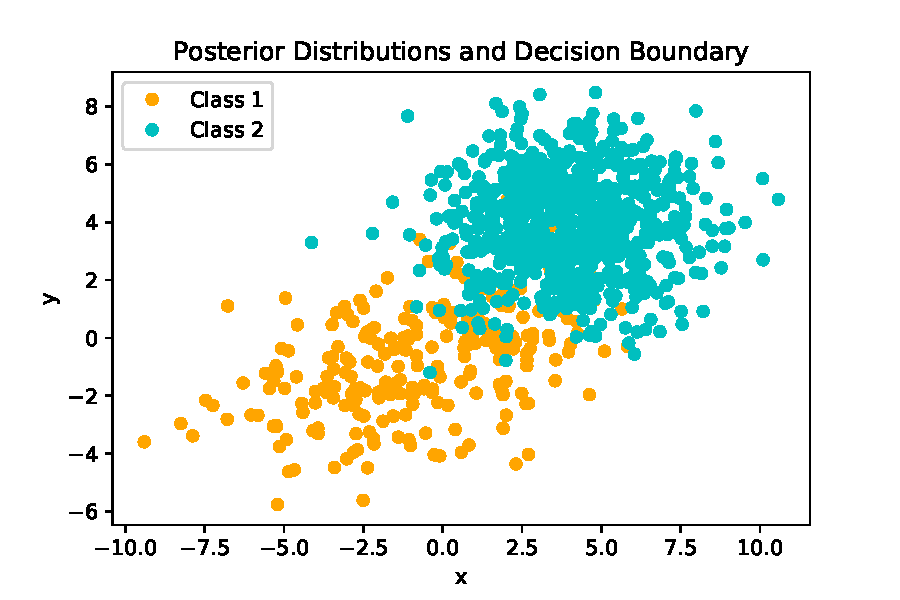
\includegraphics[scale=0.55]{04_density_estimation/02_img/pde_data_raw}
	\end{figure}
\end{frame}


% Subsection: 
% --------------------------------------------------------------------------------------------------------
\subsection{Methods for PDE}

% Overview of the Methods for PDE
\begin{frame}{Overview of the Methods for PDE}{}
	\begin{enumerate}
		\item \highlight{Parametric models} (maximum likelihood estimation)
		\begin{itemize}
			\item Assume a fixed parametric form (e.\,g. a Gaussian distribution)
			\item Estimate the parameters such that the model fits the data best
		\end{itemize}
		\item \highlight{Non-parametric models}
		\begin{itemize}
			\item Often we do not know the functional form of the density
			\item Estimate probability directly from the data without an explicit model
		\end{itemize}
		\item \highlight{Mixture models}
		\begin{itemize}
			\item Combination of \ding{182} and \ding{183}
			\item EM algorithm
		\end{itemize}
	\end{enumerate}
\end{frame}


% Section: Parametric Models
%______________________________________________________________________
\section{Parametric Models}
\makedivider{Parametric Models}

% Subsection: General Idea
% --------------------------------------------------------------------------------------------------------
\subsection{General Idea}

% General Approach
\begin{frame}{General Approach}{}
	\begin{itemize}
		\item Given some (continuous) training data $\bm{X} = \{ x^{(i)} \}_{i=1}^n$ \\
			(where all $x^{(i)}$ belong to the same class):
		\vspace*{4mm}
		\begin{figure}
			\centering
			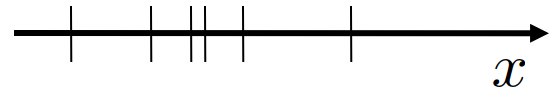
\includegraphics[scale=0.3]{04_density_estimation/02_img/pde_data_1d}
		\end{figure}
		\item Estimate $p(x)$ using a fixed parametric form:
		\vspace*{2mm}
		\begin{figure}
			\centering
			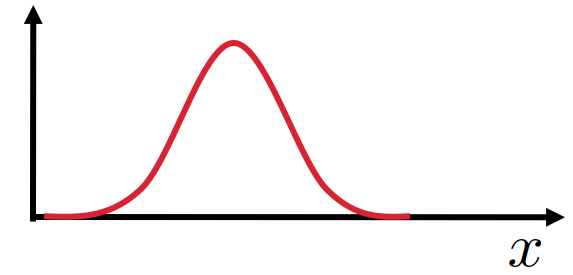
\includegraphics[scale=0.3]{04_density_estimation/02_img/pde_result_1d}
		\end{figure}
	\end{itemize}
\end{frame}


% Example: Gaussian Distribution
\begin{frame}{Example: Gaussian Distribution}{}
	\bubble{11}{10}{
		\footnotesize $\mu\ \equiv$ mean \\
		\footnotesize $\sigma^2\ \equiv$ variance
	}
	\begin{itemize}
		\item One common case is the \highlight{Gaussian distribution}:
		\begin{equation}
			p(x \vert \mu, \sigma^2) = \mathcal{N}(x \vert \mu, \sigma^2) = \frac{1}{\sqrt{2 \pi \sigma^2}}
				\exp\left\{ -\frac{(x - \mu)^2}{2 \sigma^2} \right\}
		\end{equation}
		\item Notation for parametric models:
		\begin{itemize}
			\item $p(x \vert \bm{\theta})$
			\item In the case of a Gaussian: $\bm{\theta} = \{ \mu, \sigma^2 \}$
		\end{itemize}
	\end{itemize}
\end{frame}


% Subsection: Parameter Learning and Assumptions
% --------------------------------------------------------------------------------------------------------
\subsection{Parameter Learning and Assumptions}

% Learning the Parameters
\begin{frame}{Learning the Parameters}{}
	\begin{itemize}
		\item Learning means estimating of the parameters $\bm{\theta}$ given the data $\bm{X}$
		\item \highlight{Likelihood} of the parameters $\bm{\theta}$:
		\begin{itemize}
			\item Is defined as the probability that $\bm{X}$ was generated by a
				probability density function (pdf) with parameters $\bm{\theta}$
			\begin{equation}
				\mathcal{L}(\bm{\theta}) = p(\bm{X} \vert \bm{\theta})
			\end{equation}
			\item We want to \textbf{maximize} the likelihood
		\end{itemize}
	\end{itemize}
	
	\vspace*{2mm}
	\begin{boxBlueNoFrame}
		\highlight{$\Rightarrow$ Maximum likelihood estimation (MLE)}
	\end{boxBlueNoFrame}
\end{frame}


% A fundamental Assumption
\begin{frame}{A fundamental Assumption}{}
	\begin{itemize}
		\item How to compute $\mathcal{L}(\bm{\theta})$?
		\item The data is assumed to be \highlight{i.\,i.\,d.} (independent and identically distributed):
		\begin{itemize}
			\item Two random variables $x_1$ and $x_2$ are independent, if
			\begin{equation}
				P(x_1 \le \alpha, x_2 \le \beta) = P(x_1 \le \alpha) \cdot P(x_2 \le \beta) \qquad \forall \alpha, \beta \in \mathbb{R}
			\end{equation}
			\item Two random variables $x_1$ and $x_2$ are identically distributed, if
			\begin{equation}
				P(x_1 \le \alpha) = P(x_2 \le \alpha) \qquad \forall \alpha \in \mathbb{R}
			\end{equation}
		\end{itemize}
	\end{itemize}
\end{frame}


% Subsection: Maximum Likelihood Estimation (MLE)
% --------------------------------------------------------------------------------------------------------
\subsection{Maximum Likelihood Estimation (MLE)}

% Computation of the Likelihood
\begin{frame}{Computation of the Likelihood}{}\important
	\bubble{9}{12.75}{
		\footnotesize What is the problem here?
	}
	\vspace*{-2mm}
	\begin{align}
		\mathcal{L}(\bm{\theta})
			&= p(\bm{X} \vert \bm{\theta}) \nonumber \\[2mm]
			&= p(x^{(1)}, x^{(2)}, \dots, x^{(n)} \vert \bm{\theta}) \nonumber
			\intertext{\footnotesize data is independent:}
			&= p(x^{(1)} \vert \bm{\theta}) \cdot p(x^{(2)} \vert \bm{\theta}) \cdot \ldots \cdot p(x^{(n)} \vert \bm{\theta}) \nonumber
			\intertext{\footnotesize data is identically distributed:} 
			&= \prod_{i=1}^n p(x^{(i)} \vert \bm{\theta})
	\end{align}
\end{frame}


% Computation of the Likelihood (Ctd.)
\begin{frame}{Computation of the Likelihood (Ctd.)}{}
	\bubble{11.5}{7.5}{
		\footnotesize Why is this an \\[-1mm]
		\footnotesize allowed transformation?
	}
	\bubble{4}{11}{
		$\log \Pi = \Sigma \log$
	}
	\begin{itemize}
		\item \Highlight{Problem:} Large $n$ might cause arithmetic underflows! \textbf{(why?)}
		\item Transform the likelihood using the logarithm \highlight{$\Rightarrow$ log-likelihood}
		\begin{align}
			\mathcal{L}\mathcal{L}(\bm{\theta})
				&= \log \mathcal{L}(\bm{\theta}) \nonumber \\[2mm]
				&= \log \prod_{i=1}^n p(x^{(i)} \vert \bm{\theta}) \nonumber \\[2mm]
				&= \sum_{i=1}^n \log p(x^{(i)} \vert \bm{\theta})
		\end{align}
	\end{itemize}
\end{frame}


% Maximum Likelihood of a Gaussian
\begin{frame}{Maximum Likelihood of a Gaussian}{}
	\begin{itemize}
		\item $\bm{\theta} = \{ \mu, \sigma^2 \}$
		\begin{align}
			\mathcal{L}\mathcal{L}(\{ \mu, \sigma^2 \})
				&= \sum_{i=1}^n \log \mathcal{N}(x^{(i)} \vert \mu, \sigma^2) \\
				&= \sum_{i=1}^n \log \frac{1}{\sqrt{2 \pi \sigma^2}} \exp\left\{ -\frac{(x^{(i)} - \mu)^2}{2 \sigma^2} \right\}
		\end{align}
		\item Find $\mu_{ml}$ and $\sigma_{ml}^2$ which maximize the log-likelihood:
		\begin{equation*}
			\mu_{ml}, \sigma_{ml}^2 = \argmax_{\mu, \sigma^2} \mathcal{L}\mathcal{L}(\bm{\theta})
		\end{equation*}
	\end{itemize}
\end{frame}


% Maximum Likelihood of a Gaussian (Ctd.)
\begin{frame}{Maximum Likelihood of a Gaussian (Ctd.)}{}
	\begin{itemize}
		\item Compute the partial derivatives with respect to the parameters $\bm{\theta}$
		\item Derivative w.\,r.\,t. $\mu$:
		\begin{equation*}
			\nabla_{\mu}\mathcal{L}\mathcal{L}(\bm{\theta})
				= \nabla_{\mu} \sum_{i=1}^n \log \frac{1}{\sqrt{2 \pi \sigma^2}} \exp\left\{ -\frac{(x^{(i)} - \mu)^2}{2 \sigma^2} \right\}
				= \sum_{i=1}^n \frac{x^{(i)} - \mu}{\sigma^2}
		\end{equation*}
		\item Set derivative to zero and solve:
		\begin{equation*}
			\sum_{i=1}^n (x^{(i)} - \mu) \overset{!}{=} 0
				\Leftrightarrow n \cdot \mu = \sum_{i=1}^n x^{(i)}
				\Leftrightarrow \mu = \frac{1}{n} \sum_{i=1}^n x^{(i)}
 		\end{equation*}
	\end{itemize}
\end{frame}


% Maximization of the Likelihood
\begin{frame}{Maximization of the Likelihood}{}
	\begin{figure}
		\centering
		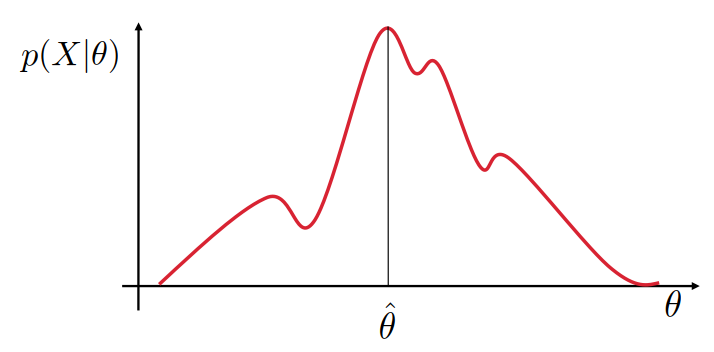
\includegraphics[scale=0.55]{04_density_estimation/02_img/maximum_likelihood}
	\end{figure}
\end{frame}


% We can classify!
\begin{frame}{We can classify!}{}\important
	\bubble{11}{4.5}{
		\footnotesize Looks familiar?
	}
	\begin{itemize}
		\item Maximum likelihood parameters:
		\begin{equation*}
			\mu_{ml} =  \frac{1}{n} \sum_{i=1}^n x^{(i)}
			\qquad\qquad
			\sigma_{ml}^2 = \frac{1}{n} \sum_{i=1}^n (x^{(i)} - \mu_{ml})^2
		\end{equation*}
		\item Now we can use Bayes' rule to predict class labels
		\begin{itemize}
			\item We have the priors...
			\item ...and the class conditionals
		\end{itemize}
		\item Also, the \highlight{decision boundary} can be computed
	\end{itemize}
\end{frame}


% Multivariate Case
\begin{frame}{Multivariate Case}{}\important
	\begin{itemize}
		\item The solution above is for 1-D data; what if we have more dimensions?
		\item \highlight{Multivariate Gaussian distribution}:
		\begin{equation}
			\mathcal{N}_D(\bm{x} \vert \bm{\mu}, \bm{\Sigma})
				= \frac{1}{\sqrt{(2 \pi)^D \vert \bm{\Sigma} \vert}}
					\exp\left\{ -\frac{1}{2} (\bm{x} - \bm{\mu})^{\intercal} \bm{\Sigma}^{-1} (\bm{x} - \bm{\mu}) \right\}
		\end{equation}
		\item Luckily, the derivations don't change:
		\begin{equation}
			\bm{\mu}_{ml} = \frac{1}{n} \sum_{i=1}^n \bm{x}^{(i)}
			\qquad
			\bm{\Sigma}_{ml} = \frac{1}{n} \sum_{i=1}^n (\bm{x}^{(i)} - \bm{\mu}_{ml}) (\bm{x}^{(i)} - \bm{\mu}_{ml})^{\intercal}
		\end{equation}
	\end{itemize}
\end{frame}


% MLE for the Example Data Set
\begin{frame}{Gaussian na\"{i}ve Bayes -- Final Model}{}
	\divideTwo{0.55}{
		\begin{figure}
			\centering
			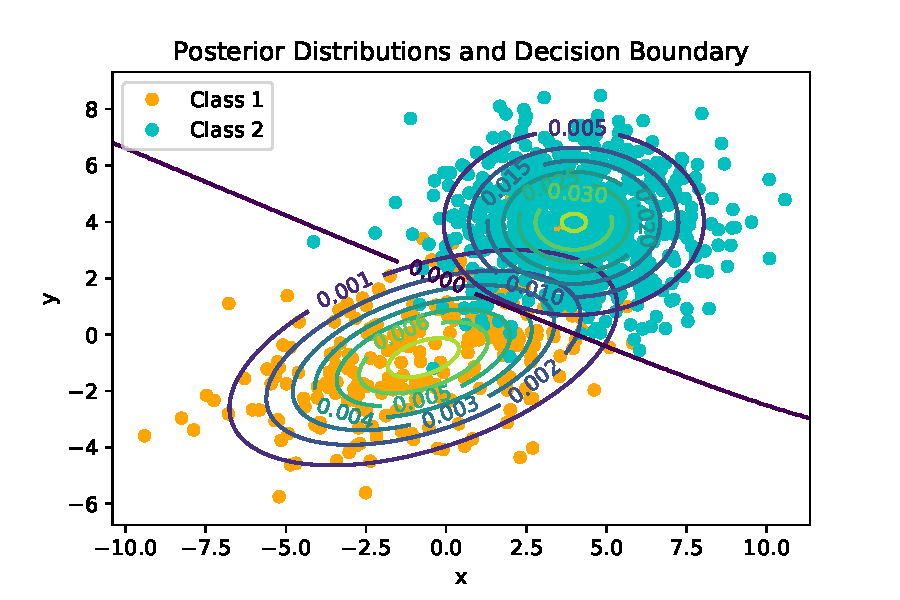
\includegraphics[scale=0.5]{04_density_estimation/02_img/pde_boundary}
		\end{figure}
	}{0.44}{
		\begin{equation*}
			\boxed{
			p(\mathcal{C}_k \vert \bm{x}) =
				\mathcal{N}_D(\bm{x} \vert \bm{\mu}_{\mathcal{C}_k}, \bm{\Sigma}_{\mathcal{C}_k}) \cdot p(\mathcal{C}_k)}
		\end{equation*}

		{\footnotesize NB: $\mathcal{N}_D(\bm{x} \vert \bm{\mu}_{\mathcal{C}_k}, \bm{\Sigma}_{\mathcal{C}_k})$ denotes the Gaussian
		distribution estimated for class $\mathcal{C}_k$ (using MLE). $p(\mathcal{C}_k)$ is the prior probability of class $\mathcal{C}_k$
		(as in the discrete case).}
	}
\end{frame}


% Section: Non-parametric Models
%______________________________________________________________________
\section{Non-parametric Models}
\makedivider{Non-parametric Models}

% Subsection: Motivation
% --------------------------------------------------------------------------------------------------------
\subsection{Motivation}

% Disadvantages of parametric Models
\begin{frame}{Disadvantages of parametric Models}{}\important
	\begin{itemize}
		\item Until now we used a fixed parametric form (e.\,g. a Gaussian) which is governed by a small amount of parameters
		\item \Highlight{This assumption may be wrong:}
		\begin{itemize}
			\item Another distribution (exponential, gamma, ...) may fit better
			\item A suitable 'text-book distribution' may not exist
		\end{itemize}
	\end{itemize}
	
	\vspace*{2mm}
	\begin{boxBlueNoFrame}
		\highlight{We don't want to make any assumptions about the underlying distribution!}
	\end{boxBlueNoFrame}
\end{frame}


% Subsection: Non-parametric Approaches
% --------------------------------------------------------------------------------------------------------
\subsection{Non-parametric Approaches}

% Non-parametric Approaches
\begin{frame}{Non-parametric Approaches}{}
	\begin{enumerate}
		\item \highlight{Histograms} (Binning)
		\item \highlight{Kernel density estimation} (KDE)
		\item \highlight{Nearest neighbors} (kNN)
	\end{enumerate}
\end{frame}


% Subsection: Histograms
% --------------------------------------------------------------------------------------------------------
\subsection{Histograms}

% Histograms
\begin{frame}{Histograms}{}
	\begin{itemize}
		\item Histograms partition the data $\bm{X} = \{ \bm{x}^{(i)} \}_{i=1}^n$ into distinct \textbf{bins} of volume $v_j$...
		\item ...and subsequently count the number of instances $k_j$ falling into the $j$-th bin
		\item Approximate the probability $p(\bm{x})$ by:
		\begin{equation}
			p(\bm{x}) \approx \frac{k_j}{n \cdot v_j}\qquad \text{for $\bm{x}$ in bin $j$}
		\end{equation}
		\item The sum of all probabilities equals 1: $\sum_{j=1}^m \frac{k_j}{n \cdot v_j} = 1$
		\item $v_j$ is a \textbf{hyper-parameter} (usually all bins have equal size) 
	\end{itemize}
\end{frame}


% Histograms (Ctd.)
\begin{frame}{Histograms (Ctd.)}{}
	\begin{minipage}{0.32\framewidth}
		\begin{center}\highlight{Too narrow}\end{center}
		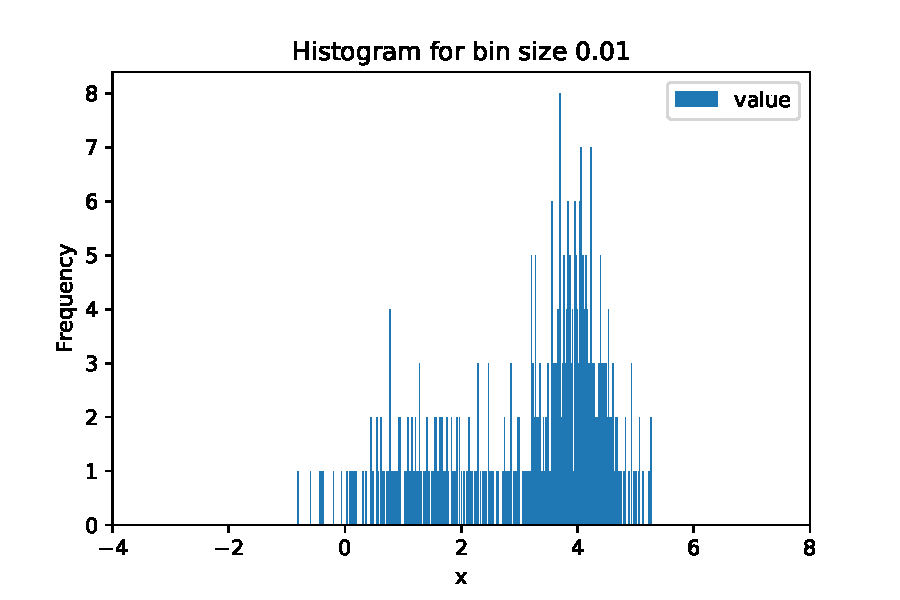
\includegraphics[scale=0.3]{04_density_estimation/02_img/histo_small}
	\end{minipage}
	\hfill
	\begin{minipage}{0.32\framewidth}
		\begin{center}\highlight{About right}\end{center}
		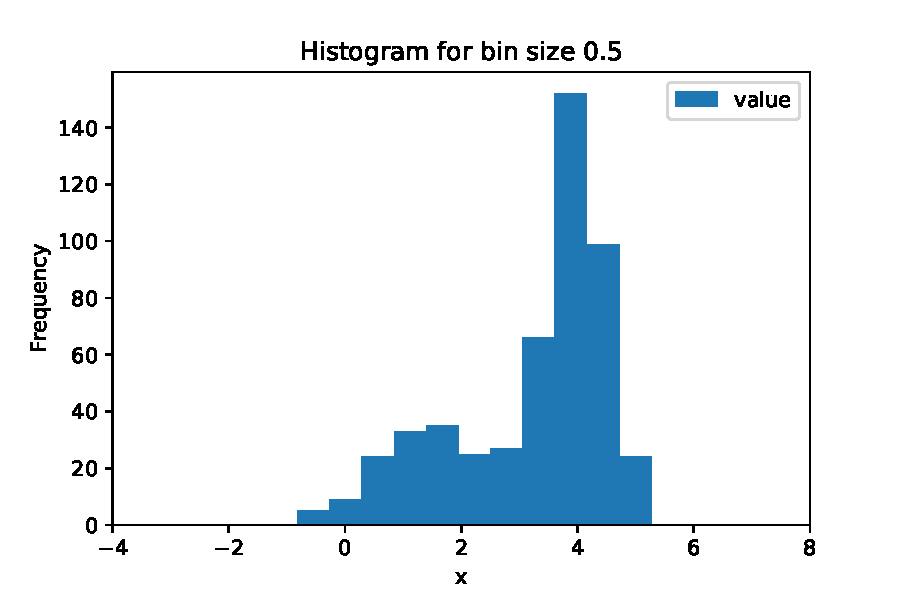
\includegraphics[scale=0.3]{04_density_estimation/02_img/histo_medium}
	\end{minipage}
	\hfill
	\begin{minipage}{0.32\framewidth}
		\begin{center}\highlight{Too wide}\end{center}
		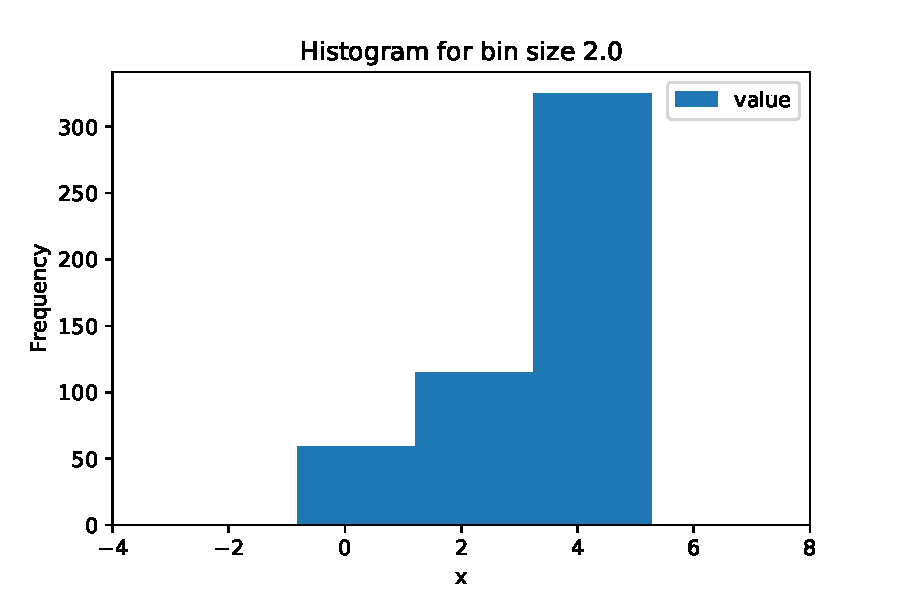
\includegraphics[scale=0.3]{04_density_estimation/02_img/histo_large}
	\end{minipage}
\end{frame}


% Drawbacks of Histograms
\begin{frame}{Drawbacks of Histograms}{}
	\divideTwo{0.55}{
		\begin{itemize}
			\item Histograms are mostly unsuited for many applications
			\item \Highlight{Drawbacks:}
			\begin{enumerate}
				\item \textbf{Discontinuities} due to bin edges
				\item Number of bins \textbf{explodes} with growing number of dimensions $D$
			\end{enumerate}
		\end{itemize}
	}{0.44}{
		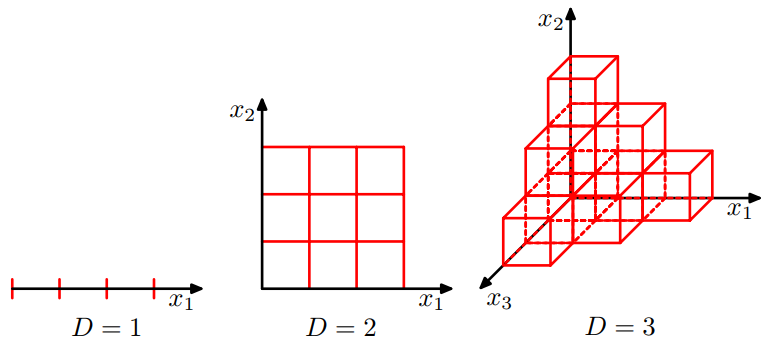
\includegraphics[scale=0.3]{04_density_estimation/02_img/curse_of_dimensionality}
	}
	
	\vspace*{4mm}
	\begin{boxBlueNoFrame}
		\highlight{The latter issue is known as the curse of dimensionality}
	\end{boxBlueNoFrame}
\end{frame}


% Subsection: Kernel Density Estimation
% --------------------------------------------------------------------------------------------------------
\subsection{Kernel Density Estimation}

% An alternative Approach
\begin{frame}{An alternative Approach}{}
	\begin{itemize}
		\item Don't use a fixed number of pre-determined bins
		\item Instead, employ a \textbf{sliding window} approach by centering a region $\mathcal{R}$ (bin)
			around the data point of interest $\bm{x}$
		\begin{equation}
			p(\bm{x}) \approx \frac{k}{n \cdot v}
		\end{equation}
		\item This gives rise to two different techniques:
		\begin{enumerate}
			\item \highlight{Kernel density estimation} (Fix $v$ and determine $k$)
			\item \highlight{k-nearest neighbors} (Fix $k$ and determine $v$)
		\end{enumerate}
	\end{itemize}
\end{frame}


% Kernel Density Estimation: Parzen Window
\begin{frame}{Kernel Density Estimation: Parzen Window}{}\important
	\begin{itemize}
		\item $\mathcal{R}$ is a $D$-dimensional \highlight{hyper-cube} of edge length $h$ centered on $\bm{x}$
		\item Determine if a data point falls into region $\mathcal{R}$:
		\begin{equation}
			H(\bm{u}) = \begin{cases} 
				1\quad \text{if}\ \vert u_d \vert \le \nicefrac{h}{2}, d = 1, 2, \dots, D \\
				0\quad \text{otherwise}
			\end{cases}
		\end{equation}
		\item The total number of data points falling into region $\mathcal{R}$ is given by:
		\begin{equation}
			k(\bm{x}) = \sum_{i=1}^n H(\bm{x} - \bm{x}^{(i)})
		\end{equation}
	\end{itemize}
\end{frame}


% Kernel Density Estimation: Parzen Window (Ctd.)
\begin{frame}{Kernel Density Estimation: Parzen Window (Ctd.)}{}\important
	\begin{itemize}
		\item The volume $v$ is simple to compute:
		\begin{equation}
			v = \int H(\bm{u}) \diff \bm{u} = h^D
		\end{equation}
		\item Putting it all together we get:
		\begin{equation}
			p(\bm{x}) \approx \frac{k(\bm{x})}{n \cdot v} = \frac{1}{n \cdot h^D} \sum_{i=1}^n H(\bm{x} - \bm{x}^{(i)})
		\end{equation}
		\item \Highlight{Problem:} \textcolor{red}{There are still discontinuities}
	\end{itemize}
\end{frame}


% Kernel Density Estimation: Gaussian Kernel
\begin{frame}{Kernel Density Estimation: Gaussian Kernel}{}\optional
	\begin{align}
		H(\bm{u})
			&= \frac{1}{\left( \sqrt{2 \pi h^2} \right)^D} \exp\left\{ -\frac{\Vert \bm{u} \Vert^2}{2 h^2} \right\} \\[1mm]
		v
			&= \int H(\bm{u}) \diff \bm{u} = 1 \\[1mm]
		k(\bm{x})
			&= \sum_{i=1}^n H(\bm{x} - \bm{x}^{(i)}) \\[1mm]
		p(\bm{x})
			&\approx \frac{k(\bm{x})}{n \cdot v} =
				\frac{1}{n \cdot \left( \sqrt{2 \pi h^2} \right)^D} \sum_{i=1}^n \exp\left\{ -\frac{\Vert \bm{x} - \bm{x}^{(i)} \Vert^2}{2 h^2} \right\}
	\end{align}
\end{frame}


% Kernel Density Estimation: Gaussian Kernel (Ctd.)
\begin{frame}{Kernel Density Estimation: Gaussian Kernel (Ctd.)}
	\begin{figure}
		\centering
		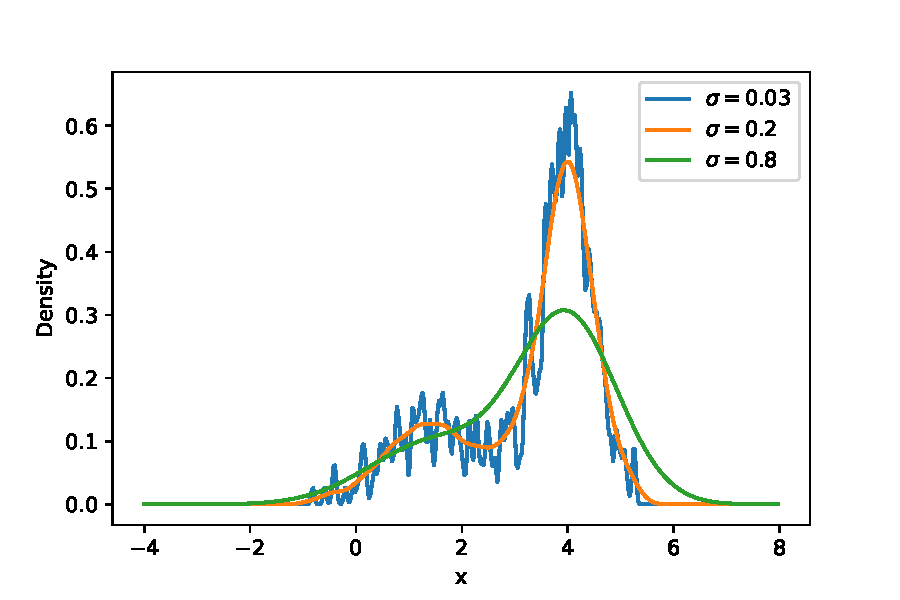
\includegraphics[scale=0.55]{04_density_estimation/02_img/kde}
	\end{figure}
\end{frame}


% Subsection: $k$-Nearest Neighbors
% --------------------------------------------------------------------------------------------------------
\subsection{$k$-Nearest Neighbors}

% k-Nearest Neighbors
\begin{frame}{$k$-Nearest Neighbors}
	\textbf{Different strategy:}
	\begin{itemize}
		\item Fix $k$ and increase the volume, until $k$ data points fall into region $\mathcal{R}$
		\begin{equation}
			p(\bm{x}) \approx \frac{k}{n \cdot v(\bm{x})}
		\end{equation}
		\item \Highlight{Usually, kernel density estimation gives better results!}
		\item We will also look at $k$-nearest neighbors as a classification method later!
	\end{itemize}
\end{frame}


% k-Nearest Neighbors (Ctd.)
\begin{frame}{k-Nearest Neighbors (Ctd.)}
	\begin{figure}
		\centering
		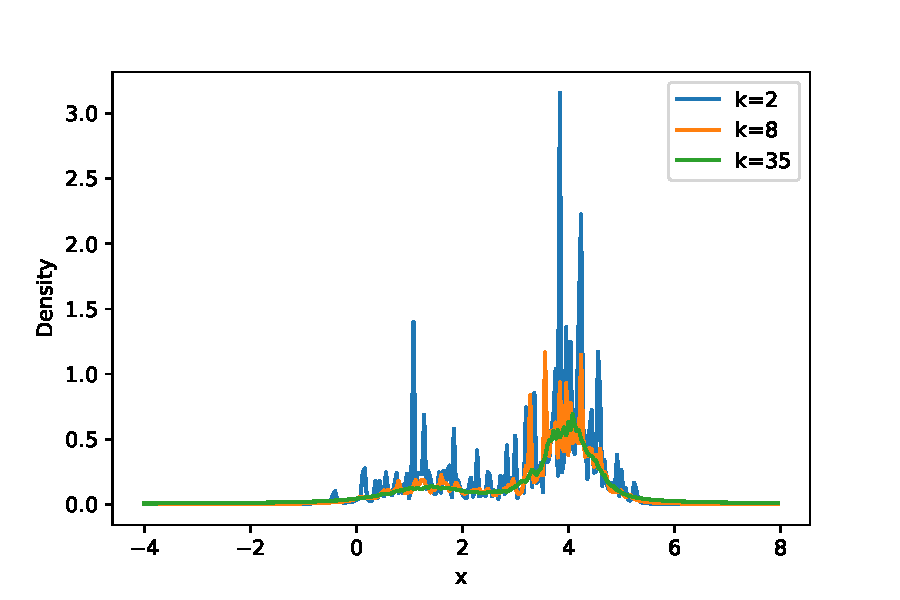
\includegraphics[scale=0.55]{04_density_estimation/02_img/knn}
	\end{figure}
\end{frame}


% Section: Mixture Models
%______________________________________________________________________
\section{Mixture Models}
\makedivider{Mixture Models}

% Subsection: General Idea
% --------------------------------------------------------------------------------------------------------
\subsection{General Idea}

% Why do we need Mixture Models?
\begin{frame}{Why do we need Mixture Models?}{}
	\begin{itemize}
		\item Parametric models have low memory footprint, are quick at runtime and often have nice analytic properties
		\item Non-parametric models make fewer assumptions about the data, but are slower and have a high memory footprint
		\item \textbf{We can combine different models in a mixture model!}
		\begin{equation}
			p(\bm{x}) = \sum_{j=1}^M p(\bm{x}|j) p(j)
		\end{equation}
	\end{itemize}
\end{frame}

% Why do we need Mixture Models? (Ctd.)
\begin{frame}{Why do we need Mixture Models? (Ctd.)}{}
	\begin{itemize}
		\item A single parametric model might fail to capture the structure of the data set \\
			\textbf{Solution:} Use more components
		\begin{figure}
			\centering
			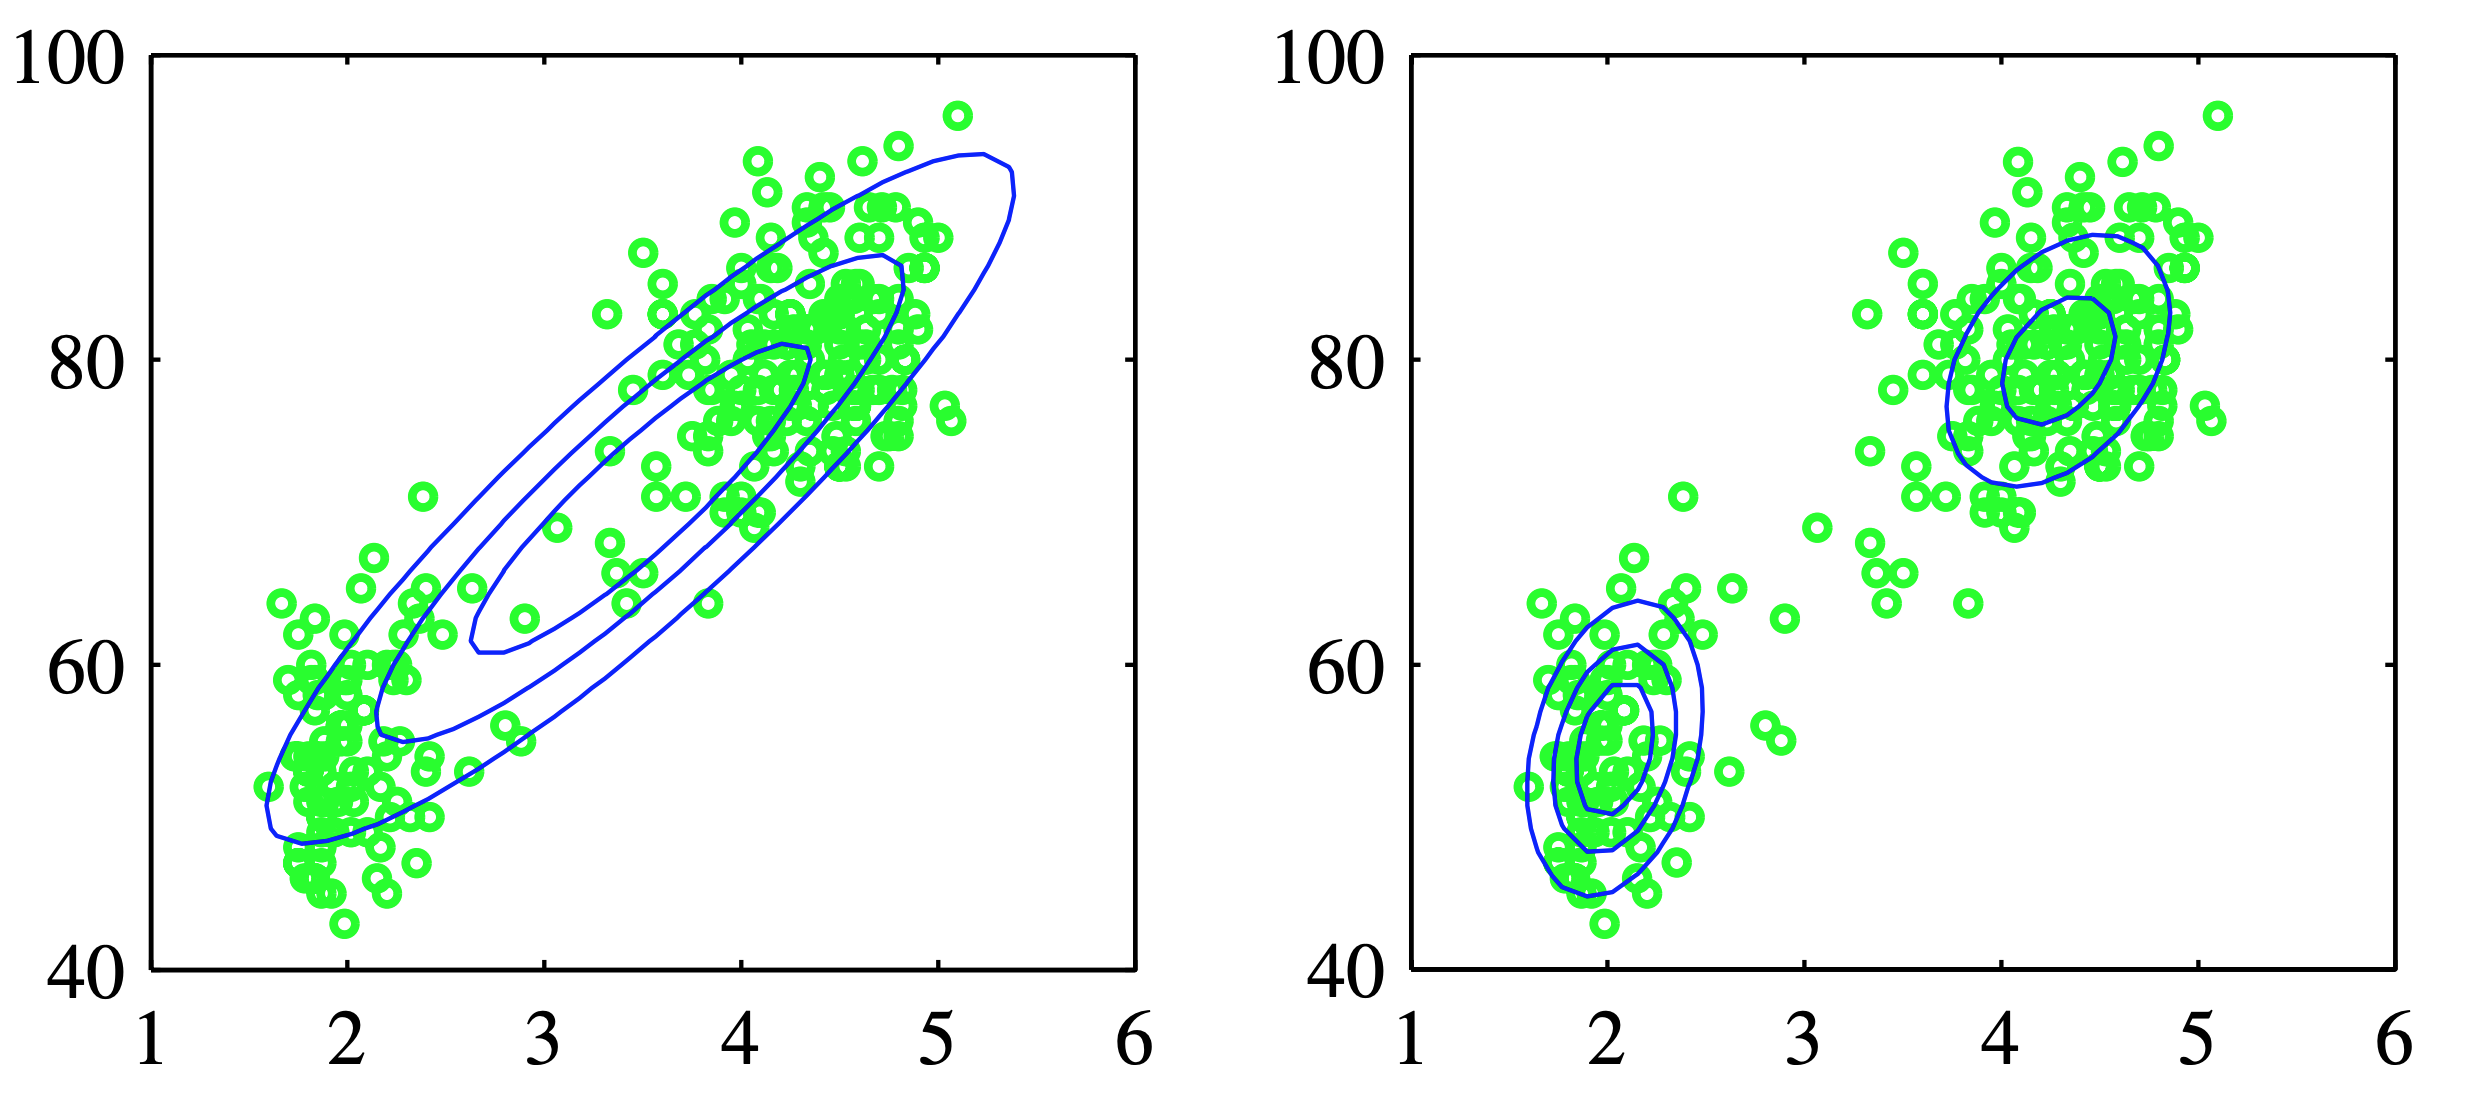
\includegraphics[scale=0.3]{04_density_estimation/02_img/mixture_models.png}
		\end{figure}
		\item Mixture distributions (e.\,g. combination of Gaussians) can approximate almost any continuous density to arbitrary accuracy (given a sufficient number of Gaussians is used)
	\end{itemize}
\end{frame}


% Subsection: Mixture of Gaussians (MoG)
% --------------------------------------------------------------------------------------------------------
\subsection{Mixture of Gaussians (MoG)}

% Mixture of Gaussians (MoG)
\begin{frame}{Mixture of Gaussians (MoG)}{}\important
	\vspace*{-3mm}
	{\footnotesize
	\begin{align}
		p(x) 
			&= \sum_{j=1}^M p(x \vert j) p(j) \qquad\text{\footnotesize \textit{probability of data given comp. $j$ $\times$ probability of comp. $j$}} \\
		p(x|j)
			&= \mathcal{N}(x \vert \mu_j, \sigma_j) = \frac{1}{\sqrt{2 \pi\sigma_j^2}} \exp \left\{ -\frac{(x - \mu_j)^2}{2\sigma_j^2} \right\} \\
		p(j) 
			&= \pi_j \qquad\text{with}\qquad 0 \le \pi_j \le 1 \qquad\text{and}\qquad \sum_{j=1}^M \pi_j = 1
	\end{align}
	
	\vspace*{-3mm}
	\textbf{Remarks:}
	\begin{itemize}
		\item The mixture density integrates to 1: $\int p(x) \diff x = 1$
		\item The mixture parameters are: $\bm{\theta} = \{ \mu_1, \sigma_1, \pi_1, \dots, \mu_M, \sigma_M, \pi_M \}$
	\end{itemize}}
\end{frame}


% Mixture of Gaussians (Ctd.)
\begin{frame}{Mixture of Gaussians (Ctd.)}{}
	\begin{figure}
		\centering
		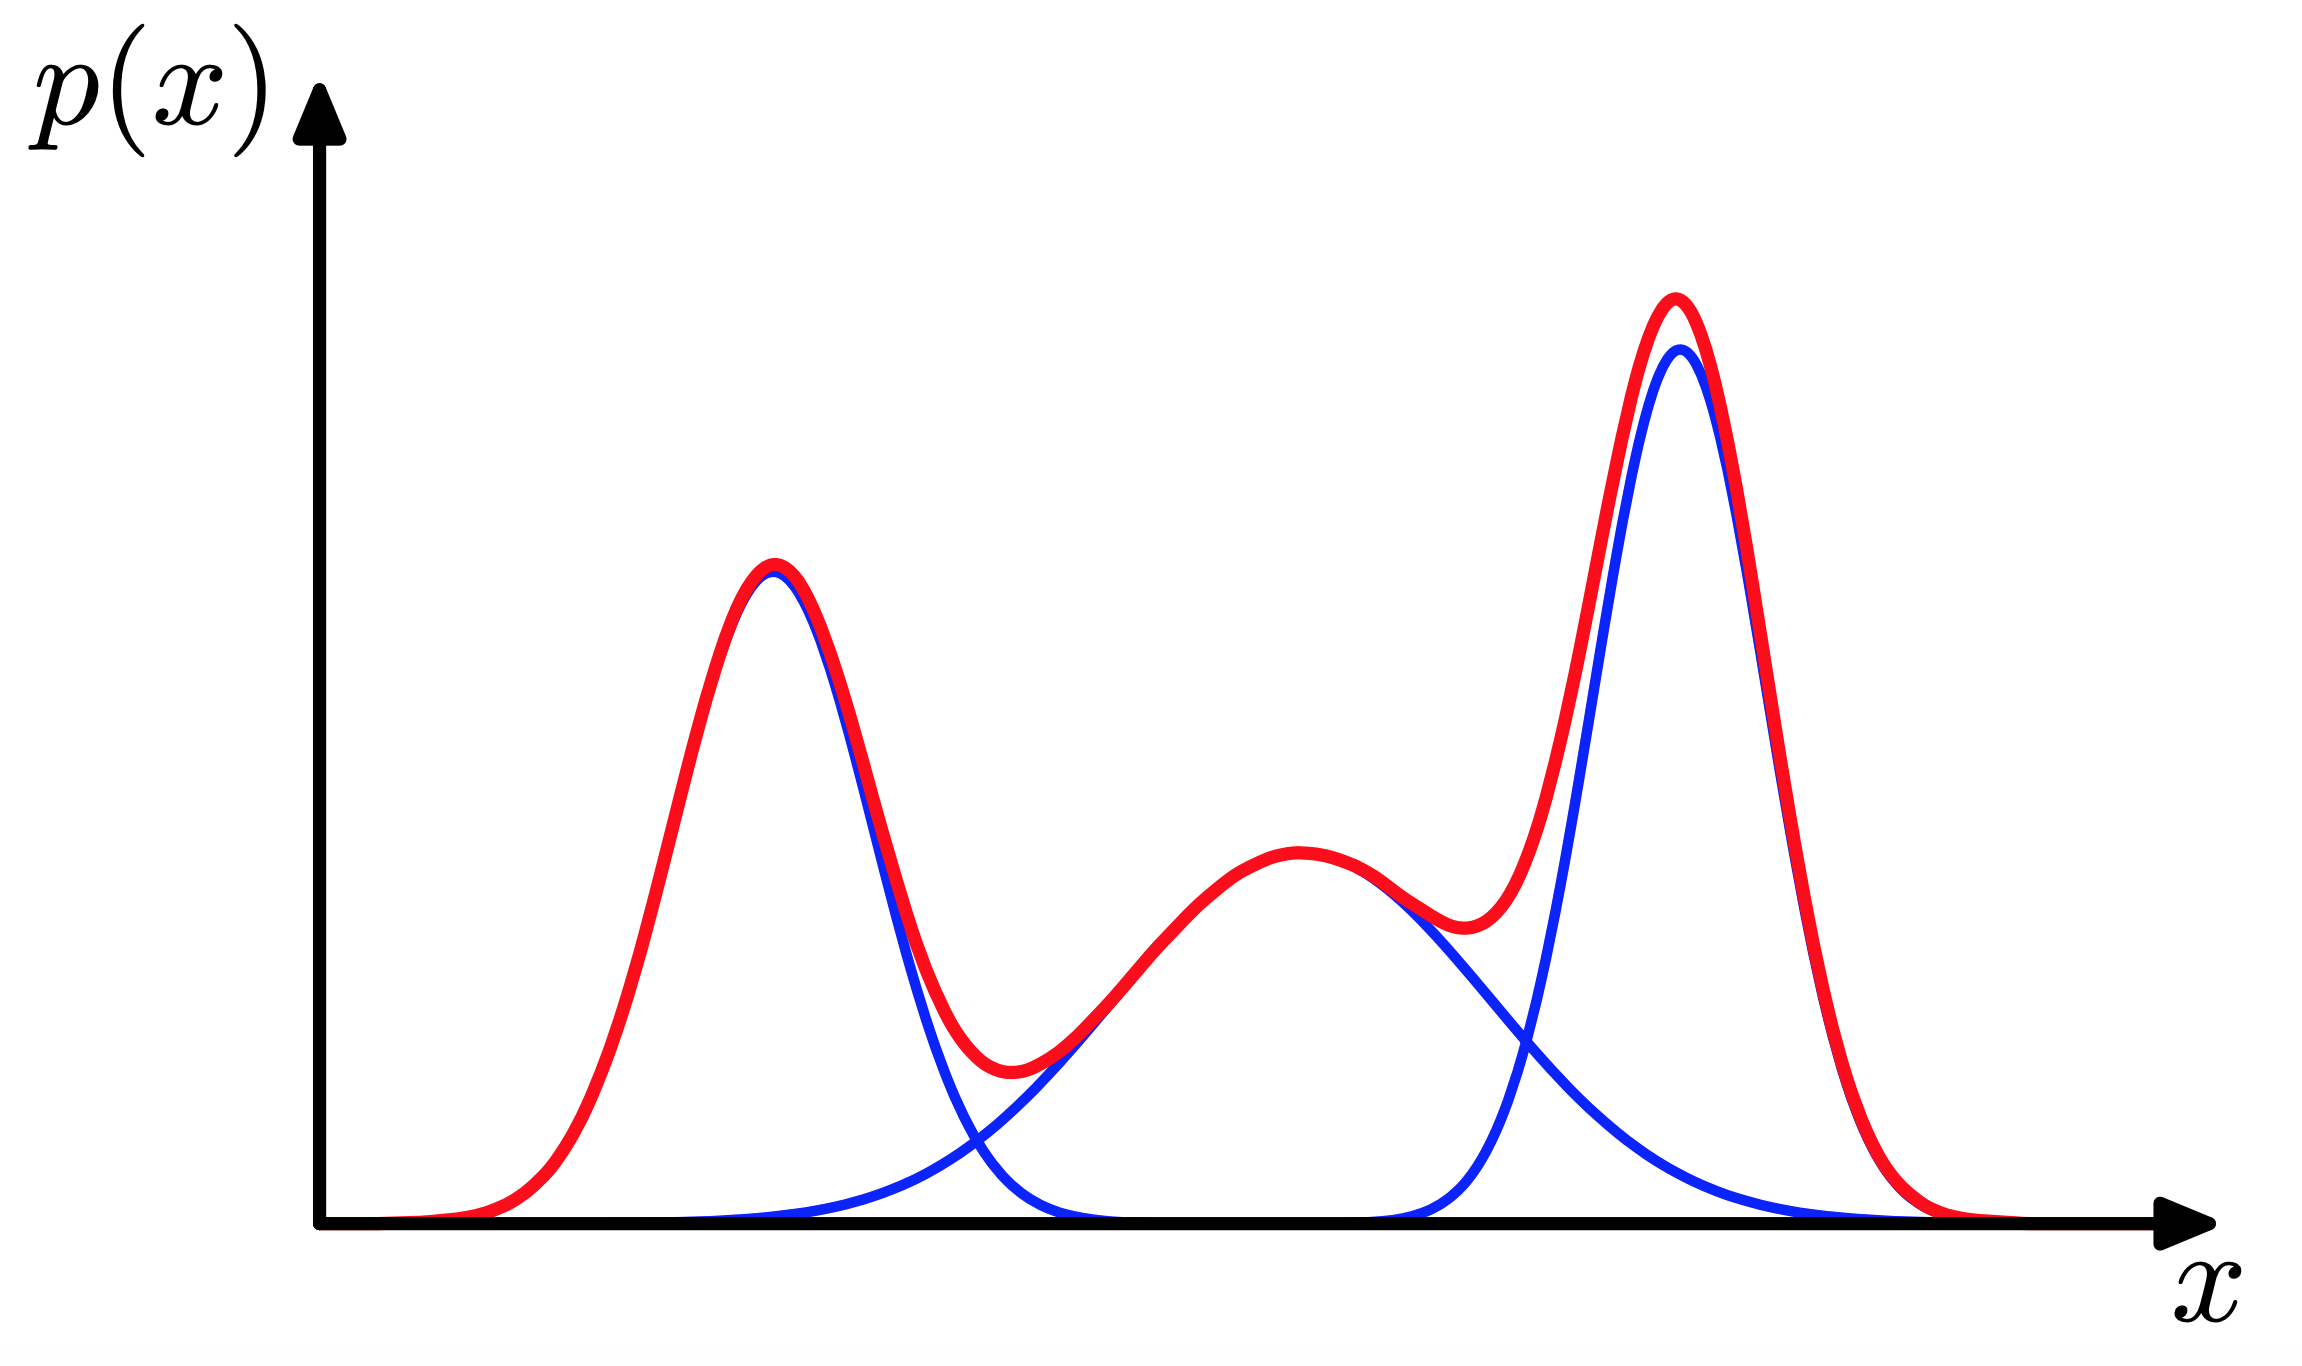
\includegraphics[scale=0.4]{04_density_estimation/02_img/gaussian_mixture}
	\end{figure}
	\vspace*{-2mm}
	\footnotesize The mixture of Gaussians \textcolor{red}{(red)} is obtained by summing over individual Gaussians \textcolor{blue}{(blue)}
\end{frame}


% Maximum Likelihood Estimation for MoG
\begin{frame}{Maximum Likelihood Estimation for MoG}{}
	\begin{itemize}
		\item We have defined our Gaussian mixture model: $p(x) = \sum_{j=1}^M p(x \vert j) p(j)$
		\item Maximize the \textbf{log-likelihood} to estimate the parameters $\bm{\theta}$:
		\begin{align}
			\mathcal{L}\mathcal{L}
				&= \log \mathcal{L}(\bm{\theta}) = \sum_{i=1}^n \log p(x^{(i)} \vert \bm{\theta}) \\[3mm]
			\nabla_{\mu_j} \mathcal{L}\mathcal{L} &\overset{!}{=} 0
			\qquad
			\mu_j = \frac{\sum_{i=1}^n p(j \vert x^{(i)}) x^{(i)}}{\sum_{i=1}^n p(j \vert x^{(i)})}
		\end{align}
		\item Do you see the issue? \Highlight{$\Rightarrow$ Circular dependency, no analytical solution!}
	\end{itemize}
\end{frame}


% Subsection: Expectation Maximization for MoG
% --------------------------------------------------------------------------------------------------------
\subsection{Expectation Maximization for MoG}

% Expectation Maximization (EM)
\begin{frame}{Expectation Maximization (EM)}{}
	\textbf{Different strategy:} We have observed data (without labels) $x^{(i)}$ and unobserved / hidden / latent variables $j \vert x$

	\begin{figure}
		\centering
		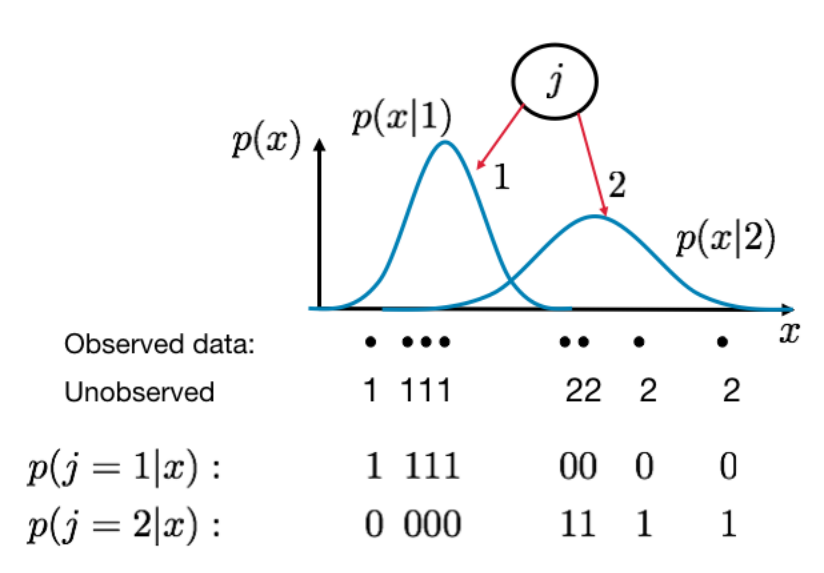
\includegraphics[scale=0.3]{04_density_estimation/02_img/em_1}
	\end{figure}
\end{frame}


% Expectation Maximization (Ctd.)
\begin{frame}{Expectation Maximization (Ctd.)}{}
	\begin{itemize}
		\item \textbf{Suppose we knew the observed and the unobserved data set:} \\
			We could compute the maximum likelihood solution of all components
		\item \textbf{Suppose we knew the distributions:} \\
			We could infer the labels for the unobserved data
		\begin{figure}
			\centering
			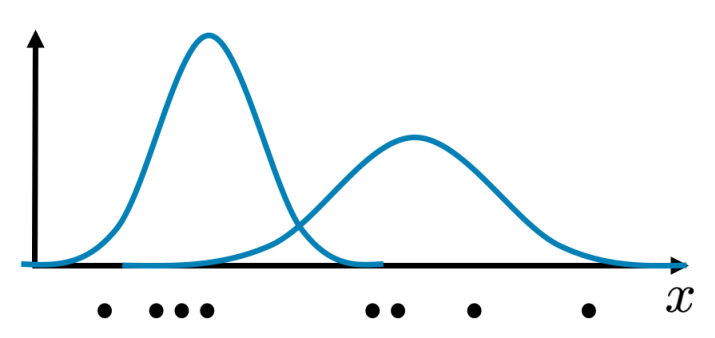
\includegraphics[scale=0.3]{04_density_estimation/02_img/em_2}
		\end{figure}
		\item \Highlight{We have neither! $\Rightarrow$ Chicken-Egg-Problem!}
	\end{itemize}
\end{frame}


% Expectation Maximization: General Procedure
\begin{frame}{Expectation Maximization: General Procedure}{}
	\begin{itemize}
		\item So, how can we estimate the mixture parameters?
		\item \highlight{EM algorithm:}
		\begin{enumerate}
			\item Start with an initial guess for the parameters
			\item \textbf{E-step:} Assign each data point $x^{(i)}$ to a component and compute $p(j \vert x^{(i)})$:
			\begin{itemize}
				\item \textit{Hard assignment:} Each data point is assigned to exactly one component  
				\item \textit{Soft assignment:} Use soft probabilities instead
			\end{itemize}
			\item \textbf{M-step:} Update the parameters based on the assignments
			\item If not converged: Go to \ding{183}
		\end{enumerate}
	\end{itemize}
\end{frame}


% Expectation Maximization: General Procedure (Ctd.)
\begin{frame}{Expectation Maximization: General Procedure (Ctd.)}{}
	\begin{figure}
		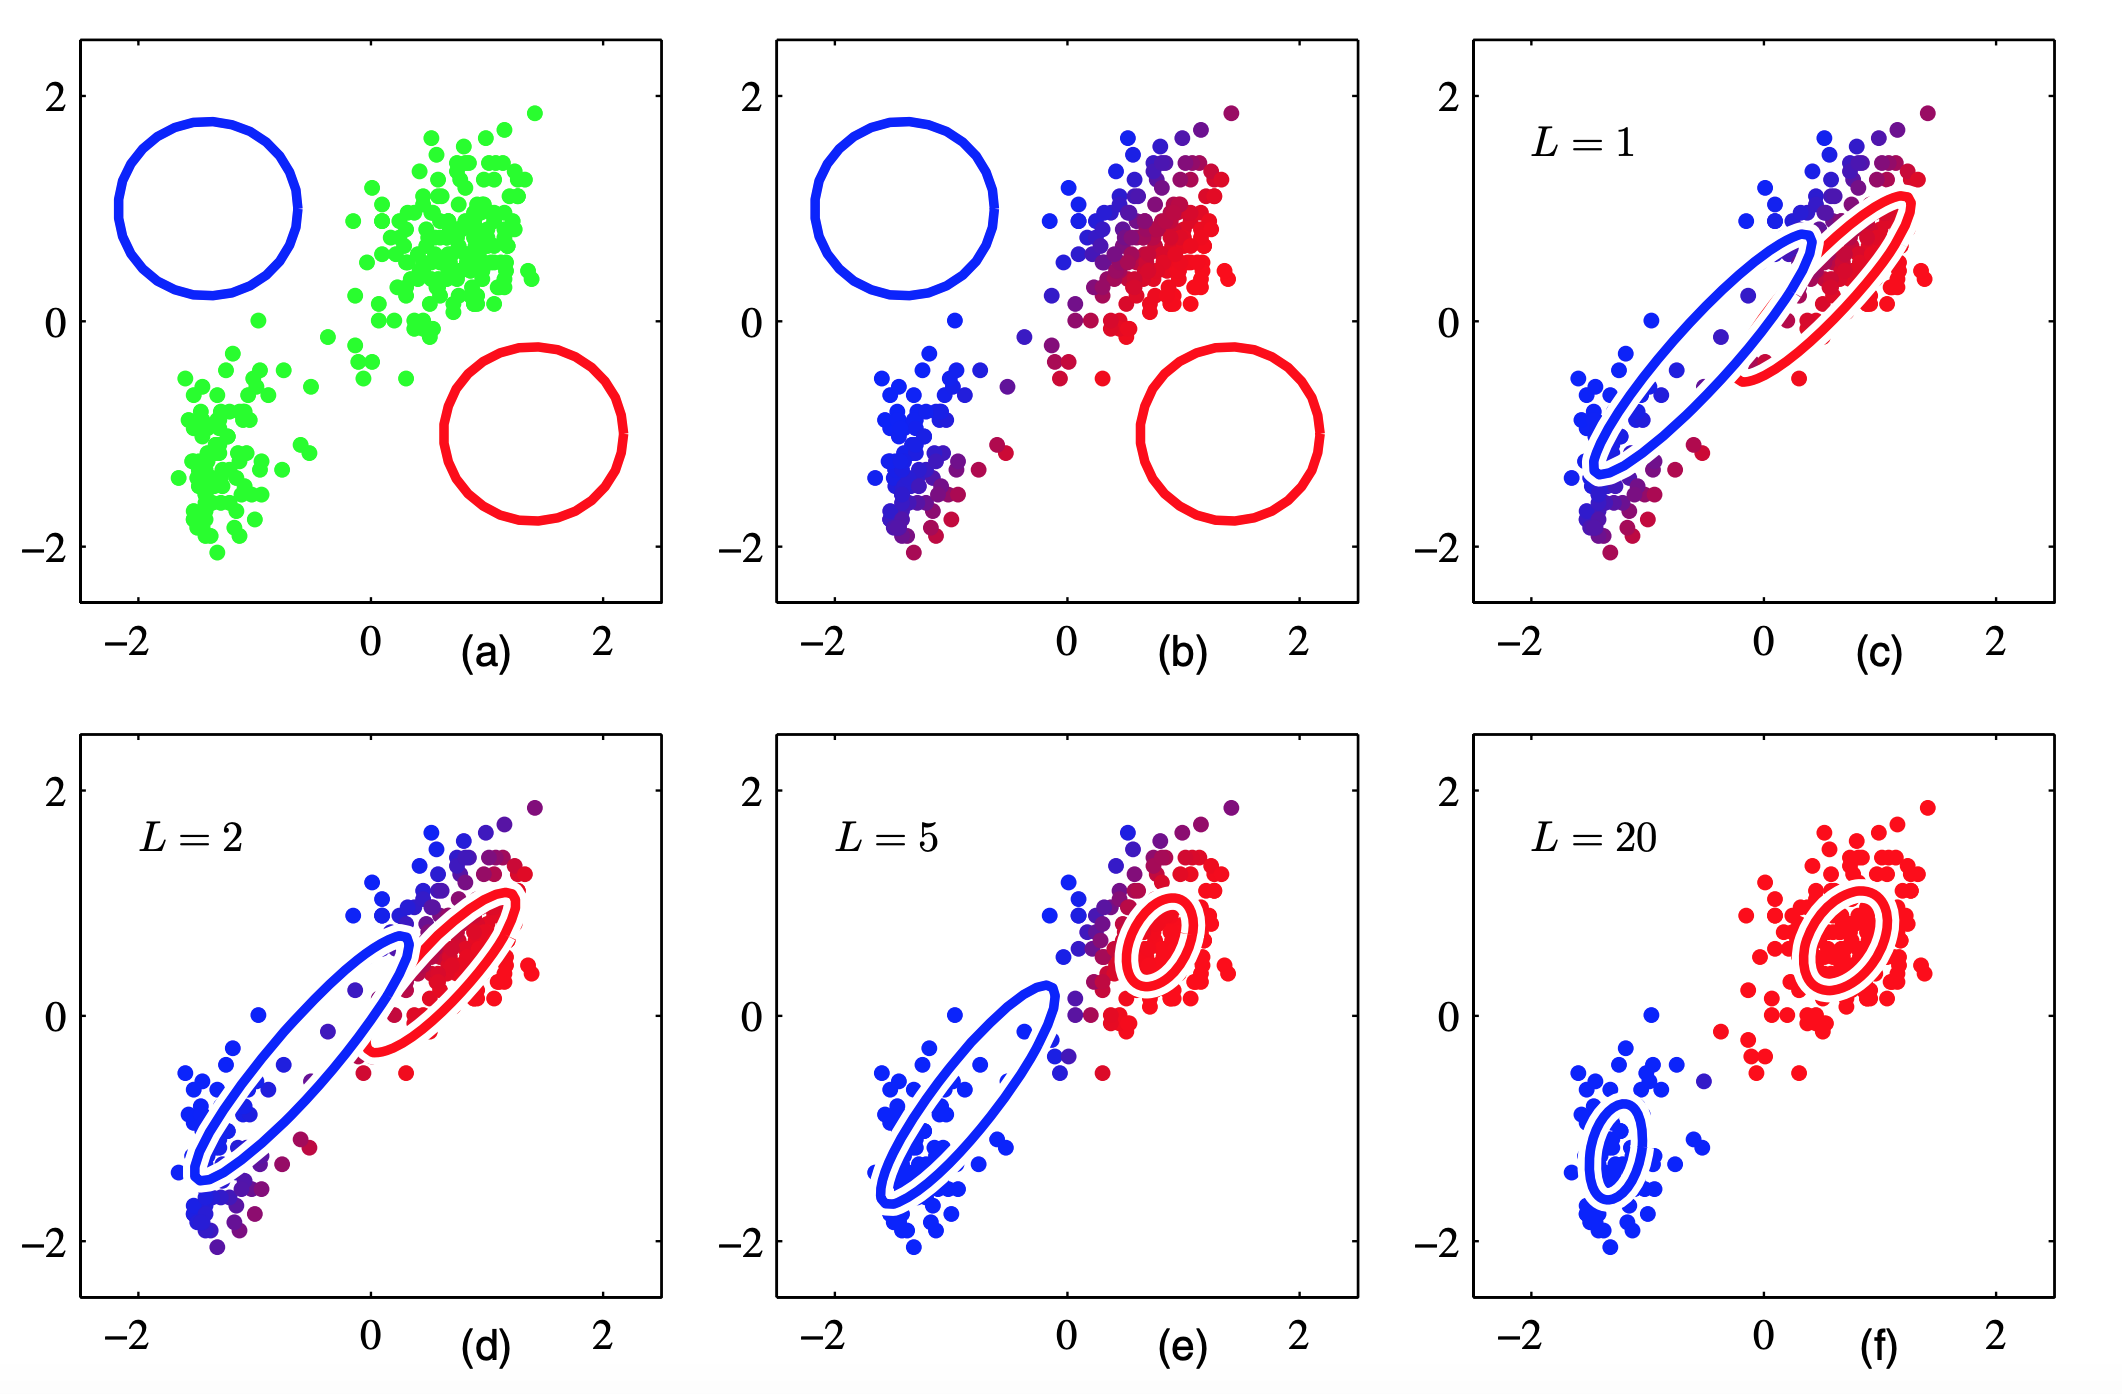
\includegraphics[scale=0.45]{04_density_estimation/02_img/em}
	\end{figure}
\end{frame}


% Expectation Maximization for MoG
\begin{frame}{Expectation Maximization for MoG}{}\important
	\vspace*{2mm}
	\textbf{EM for Gaussian Mixture Models:}
	\begin{itemize}
		\item Initialize $\mu_j, \sigma_j, \pi_j$
		\item While stop-condition is not met:
		\begin{itemize}
			\item \textbf{E-step:} Compute the posterior distribution (a.\,k.\,a. responsibility $\alpha$) for each mixture component and all data points:
			\begin{equation}
				\alpha_{ij} = p(j \vert x^{(i)}) = \frac{\pi_j \mathcal{N}(x^{(i)} \vert \mu_j, \sigma_j)}{\sum_{k=1}^M \pi_k \mathcal{N}(x^{(i)} \vert \mu_k, \sigma_k)}
			\end{equation}
			\item \textbf{M-step:} Compute new parameters using the responsibilities (cf. next slide)
		\end{itemize}
		\item Iterate until converged
	\end{itemize}
\end{frame}


% M-Step in Detail
\begin{frame}{M-Step in Detail}{}\important
	\begin{itemize}
		\item Update means:
		\begin{equation}
			\mu_j^{(new)} = \frac{1}{n_j} \sum_{i=1}^n \alpha_{ij} x^{(i)} \qquad\text{with}\qquad n_j = \sum_{i=1}^n \alpha_{ij}
		\end{equation}
		\item Update variance:
		\begin{equation}
			(\sigma_j^{(new)})^2 = \frac{1}{n_j} \sum_{i=1}^n \alpha_{ij} (x^{(i)} - \mu_j^{(new)})^2
		\end{equation}
		\item Update $\pi_j$: $\pi_j^{(new)} = \frac{n_j}{n}$
	\end{itemize}
\end{frame}


% Expectation Maximization: General Remarks
\begin{frame}{Expectation Maximization: General Remarks}{}
	\begin{itemize}
		\item \highlight{EM is a general framework and not limited to mixture models}
		\item We can use EM for performing maximum likelihood estimation, even when the data is incomplete (missing features)
		\item The log-likelihood is guaranteed to improve or stay the same in every EM iteration \highlight{$\Rightarrow$ Convergence guarantee!}
		\item Visualizations of EM for Gaussian mixture models:
		\begin{itemize}
			\item \href{https://www.youtube.com/watch?v=l1W3BvjJnmY}{\linkstyle{EM density estimation animation}}
			\item \href{https://youtu.be/eXdGCO-2n90?t=2}{\linkstyle{2-dimensional EM animation}}
		\end{itemize}
	\end{itemize}
\end{frame}


% Subsection: Recommendations
% --------------------------------------------------------------------------------------------------------
\subsection{Recommendations}

% Expectation Maximization: Some Recommendations
\begin{frame}{Expectation Maximization: Some Recommendations}{}
	\begin{itemize}
		\item \textbf{How do we initialize the parameters for EM?}
		\begin{itemize}
			\item EM depends on a good initialization of the parameters, a poor initialization can lead to bad local optima
			\item We can use \textit{k-means} to get an initial clustering
		\end{itemize}
		\item \textbf{How many mixture components do we need?}
		\begin{itemize}
			\item Use $M$ which maximizes the \highlight{Bayesian information criterion (BIC)}:
			\begin{equation}
				\log p(\bm{X} \vert \bm{\theta}_{ML}) - \frac{1}{2} K \log n
			\end{equation}
			\vspace*{-4mm}
			\begin{itemize}
				\item $K$: Number of parameters
				\item $n$: Number of data points
			\end{itemize}
		\end{itemize}
	\end{itemize}
\end{frame}



% Section: Wrap-Up
%______________________________________________________________________
\section{Wrap-Up}
\makedivider{Wrap-Up}

% Subsection: Summary
% --------------------------------------------------------------------------------------------------------
\subsection{Summary}

% Summary
\begin{frame}{Summary}{}
	\begin{itemize}
		\item We can use \textbf{parametric}, \textbf{non-parametric} and \textbf{mixture models} to estimate the density
		\item This allows us to estimate the probabilities needed by e.\,g. a na\"ive Bayes model to work with \textbf{continuous features}
		\item Parametric models assume a certain \textbf{parametric form}, e.\,g. a Gaussian
		\item \textbf{MLE} allows us to determine the parameters based on our dataset
		\item Non-parametric models directly \textbf{use the data points themselves}
		\item Use the \textbf{EM algorithm} to optimize the parameters of mixture models
	\end{itemize}
\end{frame}


% Subsection: Self-Test Questions
% --------------------------------------------------------------------------------------------------------
\subsection{Self-Test Questions}

% Self-Test Questions
\begin{frame}{Self-Test Questions}{}\important
	\begin{enumerate}
		\item What is maximum likelihood estimation? How can you get the maximum likelihood estimate for a Gaussian distribution?
		\item What does the term \textit{`non-parametric'} mean? How many parameters does such a model have?
		\item What distinguishes kernel density estimation and $k$-nearest neighbors?
		\item Why can't we use a simple maximum likelihood estimate for mixture models?
		\item What happens in the E and M steps in the EM algorithm?
	\end{enumerate}
\end{frame}


% Subsection: Lecture Outlook
% --------------------------------------------------------------------------------------------------------
\subsection{Lecture Outlook}

\begin{frame}{What's next...?}{}
	\makeoverview{5}
\end{frame}


% Subsection: Recommended Literature and further Reading
% --------------------------------------------------------------------------------------------------------
\subsection{Recommended Literature and further Reading}

% Literature
%______________________________________________________________________
\begin{frame}[allowframebreaks]{Recommended Literature and further Reading}{}
	\footnotesize
	\begin{thebibliography}{2}
		\literature{book}{Bishop.2006}{[1] Pattern Recognition and Machine Learning}
			{Christopher Bishop. Springer. 2006.}{$\rightarrow$ \href{
				http://users.isr.ist.utl.pt/~wurmd/Livros/school/Bishop\%20-\%20Pattern\%20Recognition\%20And\%20Machine\%20Learning\%20-\%20Springer\%20\%202006.pdf
			}{\linkstyle{Link}}, cf. chapters 1.2.4, 2.5, 9.2}
	\end{thebibliography}
\end{frame}


% Subsection: Meme of the Day
% --------------------------------------------------------------------------------------------------------
\subsection{Meme of the Day}

% Meme of the Day
\begin{frame}{Meme of the Day}{}
	\begin{figure}
		
\includegraphics[scale=0.90]{04_density_estimation/02_img/gaussianseverywhere}
	\end{figure}
\end{frame}


% Thank you
%______________________________________________________________________
\makethanks

\end{document}